\documentclass[12pt, reqno]{amsart}
% \pdfoutput=1



% Packages to open
\usepackage{amsthm, amssymb, amsmath, enumerate}
% \usepackage{fullpage}
\usepackage{verbatim}
\usepackage{graphicx, graphics}
\usepackage{algorithm}
\usepackage{longtable}
\usepackage{cancel}


% Setup TikZ

\usepackage{tikz}
\usetikzlibrary{arrows}
\tikzstyle{block}=[draw opacity=0.7,line width=1.4cm]

% Hopefully dot packages
\usepackage[all,arc,curve,frame,color]{xy}
\usepackage{subfigure}
\usepackage{url, hyperref}


% \usepackage{setspace}  % Use command \doublespacing or \onehalfspacing

% Standard Theorem Styles
\newtheorem{thm}{Theorem}[section]
\newtheorem{lem}[thm]{Lemma}
\newtheorem{cor}[thm]{Corollary}
\newtheorem*{cor*}{Corollary}
\newtheorem{prop}[thm]{Proposition}
\newtheorem{obs}[thm]{Observation}
\newtheorem{claim}[thm]{Claim}
\newtheorem*{conjecture*}{Conjecture}
\newtheorem{conjecture}[thm]{Conjecture}
\newtheorem*{thm*}{Theorem}

\theoremstyle{remark}
\newtheorem*{question*}{Question}
\newtheorem{question}[thm]{Question}
\newtheorem{answer}[thm]{Answer}
\newtheorem{remark*}[thm]{Remark}
\newtheorem{example}[thm]{Example}

\theoremstyle{definition}
\newtheorem{define}[thm]{Definition}
\newtheorem*{define*}{Definition}
\newtheorem{idea}{Idea}
\newtheorem{problem}{Problem}
\newtheorem{exercise}[thm]{Exercise}

\numberwithin{equation}{section}  % number equations by section

% Standard shortcuts
\newcommand{\LL}{\mathcal{L}}     % Fancy script L
\newcommand{\MM}{\mathcal{M}}  % Fancy script M
\newcommand{\OO}{\mathcal{O}}    % Fancy script O
\newcommand{\FF}{\mathbb{F}}      % Finite field
\newcommand{\ZZ}{\mathbb{Z}}     % Integers
\newcommand{\RR}{\mathbb{R}}     % Reals
\newcommand{\PP}{\mathbb{P}}      % Projective space
\newcommand{\Aff}{\mathbb{A}}      % Affine space
\newcommand{\XX}{\mathcal{X}}      % Model of a variety - script X
\newcommand{\QQ}{\mathbb{Q}}      %Rationals
\newcommand{\CC}{\mathbb{C}}      % Complex Numbers
\newcommand{\mm}{\mathfrak{m}}   % maximal ideal
\newcommand{\pp}{\mathfrak{p}}   % prime ideal
\newcommand{\qq}{\mathfrak{q}}  % another prime ideal
\newcommand{\Gm}{\mathbb{G}_m}  % blackboard bold G for the multiplicative group
\newcommand{\hh}{\mathfrak{h}}  % Upper half plane
\newcommand{\tab}{\hspace{.4cm}} % Tab 



 % Color comments!
\usepackage{xcolor}
% Color comments



%Notes to ourselves
\newcommand{\diane}[1]{{\color{magenta} \sf $\clubsuit\clubsuit\clubsuit$ Diane: [#1]}}
\newcommand{\michelle}[1]{{\color{orange} \sf $\clubsuit\clubsuit\clubsuit$ Michelle: [#1]}}


% Some regularly used operator shortcuts
\newcommand{\Hom}{\operatorname{Hom}}
\newcommand{\im}{\operatorname{im}} % Image
\newcommand{\coker}{\operatorname{coker}}  % Cokernel
\newcommand{\Sym}{\operatorname{Sym}}      % Symmetric product
\newcommand{\Spec}{\operatorname{Spec}}
\newcommand{\ord}{\operatorname{ord}}
\newcommand{\Div}{\operatorname{div}}    % Divisor of a rational function
\newcommand{\Gal}{\operatorname{Gal}}  % Galois group
\newcommand{\Gauss}{\operatorname{Gauss}}  % Used for the Gauss point
\newcommand{\supp}{\operatorname{supp}}   % Support
\newcommand{\Pic}{\operatorname{Pic}}        % Picard Groups
\newcommand{\Jac}{\operatorname{Jac}}       % Jacobian Variety
\newcommand{\mult}{\operatorname{mult}}  % multiplicity
\newcommand{\pr}{\operatorname{pr}}     % projection
\newcommand{\sep}[1]{{#1}^{\operatorname{s}}}    % separable closure
\newcommand{\Spf}{\operatorname{Spf}}    % formal spectrum
\newcommand{\Frac}{\operatorname{Frac}}    % Fraction field
\newcommand{\chern}[1]{c_1\left(#1\right)}   % First Chern class
\newcommand{\codim}{\operatorname{codim}}  % codimension
\newcommand{\dist}{\operatorname{dist}}   % distance
\newcommand{\an}[1]{\operatorname{an}}  % analytic space notation
\newcommand{\Aut}{\operatorname{Aut}}   % Automorphism group
\newcommand{\Rat}{\operatorname{Rat}}    % space of rational maps
\newcommand{\PGL}{\operatorname{PGL}}
\newcommand{\PSL}{\operatorname{PSL}}
\newcommand{\alg}[1]{{\overline{#1}}}
\newcommand{\GG}{\mathbb{G}}


% Miscellaneous notational shortcuts
\newcommand{\leftexp}[2]{{\vphantom{#2}}^{#1}{#2}}   % Superscript on the left
\newcommand{\simarrow}{\stackrel{\sim}{\rightarrow}}    % Isomorphic mapping
\newcommand{\ip}[2]{\left\langle #1,#2 \right\rangle} %inner product
\newcommand{\into}{\hookrightarrow}     % Inclusion arrow
\newcommand{\dint}{\int \!\!\! \int}   % double integral
\newcommand{\tth}{^{\operatorname{th}}}
\newcommand{\Berk}{\mathbf{P}}  % Berkovich Projective Space

\newcommand{\Manoa}{M\=anoa}
\newcommand{\Hawaii}{Hawai\kern.05em`\kern.05em\relax i}
\newcommand{\Hokulea}{H\=ok\=ule\kern.05em`\kern.05em\relax a}


% Document Specific Declarations
\newcommand{\id}{\mathrm{id}}
\newcommand{\oo}{\mathfrak{o}}
\DeclareMathOperator{\Per}{Per}
\DeclareMathOperator{\PrePer}{PrePer}
\DeclareMathOperator{\Twist}{Twist}
\DeclareMathOperator{\Ker}{Ker}


%%%%%%%%%%%%%%

\title{Math 111 :  Course Outline}





%%%%%%%%%%%%%%


\begin{document}


\maketitle

This document contains suggestions for running a Math 111 class in ways that have proven  successful in the past.  All of the ideas here should be understood as descriptions of what's been done and suggestions of what you might try, and nothing more.  

Four chapters make up the Math 111 course materials:
\begin{enumerate}
\item
Problem Solving (about 3 weeks)
\item
Place Value (about 3 weeks)
\item
Number and Operations (about 4--5 weeks)
\item
Fractions (about 5--6 weeks)
\end{enumerate}

The chapters are intended to be used in this order, though there is certainly flexibility.  If you have a favorite topic or lesson not represented in these chapters, you should definitely use it.  Perhaps you want to incorporate some history of mathematics or some ethnomathematics.  These would be wonderful experiences for your students!  

Be aware that the planned chapter for Math 112 include:
\begin{enumerate}
\item
Patterns and Algebra 
\item
Fractions and Decimals
\item
Geometry 
\end{enumerate}



You will probably  alter these suggested timelines as it suits your style and the needs of your class. 
If you feel students are struggling or just not getting one particular topic, it may not be fruitful to stick with it and insist on mastery by the whole class.  Remember that we are trying to provide students with the tools to \emph{eventually} develop profound understanding of fundamental mathematics, but we do not believe we can get them there in a semester or a year.  Use your professional judgment about when it is worth spending more time, when  to move on, and when to skip sections entirely.

The materials include reading for the students, activities for in-class use, and problem banks.  Some chapters will include suggestions for self-checks on procedural skills, since these are assumed as background knowledge.  As an instructor, you may wish to require that students submit to you proof of passing such assessments, or you may want to supplement the materials with some skills practice if you deem it necessary for the majority of your students.


A typical class might proceed as follows:
\begin{itemize}
\item
Whole-class discussion about a homework problem or  reading.  To start the discussion,  a student  presents her solution to the problem or summarizes what was discussed in the reading.
\item
Think/pair/share\footnote{This is a standard methodology used in inquiry-based learning.  Read a description here: \url{http://theiblblog.blogspot.com/2011/08/classroom-strategy-think-pair-share.html}.} for a launch activity.   These are labeled in the materials under this heading.
\item
Call on individuals or groups to present their work.  Depending on the activity, there may be just one presentation or more than one.  (You may want to give the groups a few minutes notice so they can prepare what to say.)  Emphasize that these presentations are launch points for a class discussion, so students are not expected to give polished solutions after a partial class period.
\item
Debrief the launch activity.  This may include student presentations or a short instructor   lecture on key ideas.  (In an IBL class, the content marked ``Definition'' or ``Example'' in the student materials should grow out of student work on the ``Think / pair / share'' activities and the problems rather than assigned as readings during class.   Including these materials in the text is intended to give students a reference for later study.  Working on and presenting problems, not reading the text, should be the main activity during class time.)
\item
The rest of class will vary depending on the activity and the class: Students may continue working on the problem with the expectation of finishing a good write-up by the end of class or for homework.  There may be a short quiz or other individual assessment.  Students may read from the course materials and then work on a problem or  another Think/pair/share activity. 
\end{itemize}

For most Math 111 classes, there will be a lot of group work both in and out of class.  Students will often collaborate on their homework, though instructors should insist that write-ups are individual work except on assignments that are explicitly assigned to groups.    Weaker students may be inclined to defer to group members rather than assert themselves to ask questions and make sure they follow along. 

 As an instructor, you can look out for these situations as the groups are working, check in with individual students, and help the groups take responsibility for all members' understanding.  (One method: call randomly on students to present and assign a score to the group based on the quality of that presentation.  It is therefore in the group's best interest to insure that everyone participates and understands the solution.)

In addition to helping the groups as they work, it is useful to have regular individual assessments.  Quizzes and  ``exit tickets''\footnote{Usually this is a short, often anonymous, questionnaire done at the end of class that students must turn in before leaving.  Typical questions: ``One thing I understand from today's class is \underline{
\qquad\qquad\qquad}.  One thing I do not understand well is \underline{
\qquad\qquad\qquad}.  One question or concern I have is \underline{
\qquad\qquad\qquad}.''   You can read other ideas here: \url{http://www.adlit.org/strategies/19805/}.}  can help you identify students who are struggling and help these students see for themselves how they are doing.


\subsection*{Choice of content}
The content for Math 111 / 112 was selected to align with the Common Core State Standards\footnote{\url{http://www.corestandards.org/Math}} for grades K--5.  Some content that appears in many ``Math for Elementary Teachers'' textbooks is not included in these materials, because it does not appear in the K--5 curriculum.  This includes:
\begin{itemize}
\item 
Integers (negative numbers)
\item
Ratio and proportion
\item
Prime factorization, gcf, and lcm
\end{itemize}

Our intent is to focus on depth of coverage for the K--5 curriculum and on the process of doing mathematics and justifying solutions, 
rather than rushing to cover many more topics.  

We encourage you to spend time in class letting students struggle and find their own way.  Ask questions rather than explaining.  Remember that your students will eventually have to make sense of mathematical ideas without your guidance.  They will have to become the mathematics experts in their own classrooms.  It is far more important that we affect their view of mathematics and of themselves as learners and doers of mathematics than that we cover any particular piece of the elementary curriculum.


\subsection*{Notation}
The student materials use notation like $>$, $<$, and fractions without comment.  We assume these ideas are familiar to students, even if they are perhaps a bit fuzzy.  Through repeated exposure to the ideas, working in collaborative groups to help unpack meaning and fill in the gaps, this notation will become second nature.

The use of variables to express relationships rather than as ``unknowns'' where we solve an equation is really at the heart of algebra.  But most students' algebra backgrounds have focused on procedural questions (solve for $x$) rather than structural ideas (write an expression to describe this relationship).  Carolyn Kieran found that when students were asked to express the meaning of $a+3$, they couldn't because there is no equals sign and no number on the other side.

By using variables in this more procedural way throughout the course, we in fact will bolster students' overall algebra skills and their ability to (in the words of the Common Core State Standards) ``reason abstractly and quantitatively.''   We encourage you to reinforce this use of algebra in your students' work.  Ask them to give names to quantities when they want to refer to them, ask how something could be written in symbols, and so on.  This is part of our mathematical language, and through use (not through repeated dill exercises), students will acquire the language more naturally and become fluent in its use.




\newpage

\section{Chapter 1: Problem Solving}
Starting with the ``Problem Solving'' chapter allows you to set the tone for the class.  The message to students is intended to be:

\begin{itemize}
\item
Mathematics is about solving problems and explaining your work to others.
\item
You should always be able to explain \emph{why} your answer is correct for any mathematical problem (or exercise).
\end{itemize}

Most of the problems in this chapter require little mathematical background, though some of them use ideas which some students may find ``familiar but forgotten''  (examples: prime numbers, the symbols $<$ and $>$, use of variables in explanations, and so on.)   


This is intentional. The reason for couching many of the activities in the ``Think/pair/share'' structure is twofold:
\begin{enumerate}
\item
It creates a classroom atmosphere in the first few weeks that insists on students talking to each other about mathematics, and
\item
it encourages students to ask clarifying questions without fear of reproach.
\end{enumerate}
It also reinforces the idea that a mathematical problem doesn't ask you what you already know.  Sometimes, in working on a problem, you need to build some mathematical background (or remind yourself of it) in order to proceed.  Many of the ideas will appear in later chapters, so there's no need to spend a lot of time on them now.  

Reassure students (and yourself) that if they're not quite solid on some of the ideas discussed in class, they'll have opportunities to master them when those ideas come back around.  The focus is on building a collaborative environment and developing a toolbox of problem solving strategies.

The chapter contains a short warm-up activity, followed by seven sections:
\begin{description}
\item[Problem or Exercise?] This short in-class activity is designed to help students understand the difference between building skills and solving mathematical problems.  Both activities are important, but the point of the skill-building is to improve our ability to solve problems and reason carefully.   Basic skills themselves are not the end-goal of learning mathematics. 

\item[Problem Solving Strategies] Used as in-class activities, this could take several days of class.  Alternately (and maybe preferably?) your students can generate their own list of strategies by working on problems in class.  After each problem, encourage students to articulate how they solved it, and especially how they got started.  You might wish to keep a running list of your students' own problem-solving strategies, either on the board or a poster or online where students can access it an add to it.  The whole section could then be a homework reading assignment \emph{after} students have created their own list of strategies.

\item[Beware of Patterns!] This is an optional section, but we have found that students (and practicing teachers) tend to believe that if an ``obvious'' pattern fits a problem, then that pattern simply must continue.  This section is designed to dispel that myth through a surprising ``pattern-breaking'' problem.  The remainder of the section focuses on tying apparent patterns back to the problem context.  It may be heavy-going for some classes early in the term, and may best be left to a later date.

\item[Problem Bank] These problems are intended to be used for homework or additional in-class work.  There are too many problems here, so do not expect or plan to have students tackle them all!  The idea is to pick-and-choose (or to allow students to do so).  We also have a suggestion for using these problems as part of a whole-class writing activity.  See later in these notes for ideas.  You may even wish to continue assigning problems from this section as students work through the other three chapters, to keep problem solving as a major theme in the course.

\item[Careful Use of Language in Mathematics] The focus throughout the entire Math 111 / 112 course is on sense-making and explaining mathematics.  This requires students to develop better mathematical language skills.  This section starts them on that path.  These ideas should be covered at some point during Math 111, but could be put off until they come up more naturally in class.  This is a text-heavy section, so look for ways to make it more interactive and engaging.  For example, in the ``All About the Benjamins'' problem, you want to create envelopes with Monopoly money (or just slips of paper, though you'll need to change the statements accordingly) and have volunteers justify to the class whether the given statements are true or false.

\item[Explaining Your Work] Clear communication is essential in all mathematics classes, but it is especially important that future teachers develop the ability to explain mathematical ideas well.  The activity presented of critiquing student work on a problem  is particularly powerful, and one we suggest using with regularity (drawing on your own students' work).  Looking at other students' work with a critical eye helps students begin to do the same with their own work.  See the notes below for an additional writing activity to accompany this section.  This section could also be put off until a later point in class, when you begin requiring students to write more explanations and justifications.  It is perfectly fine to keep the first chapter short and focused on the idea of solving problems rather than on the write-ups.

\item[The Last Step] This section encourages students to become not just problem solvers but also problem posers.  Getting in the habit of asking questions is powerful for mathematics learners, especially since they will probably quickly stumble upon unsolved or very difficult problems if they do this.  Again, the hope is to develop the capacity for asking ``what if'' questions in these future teachers, in the hope that they encourage questioning and curiosity about mathematics in their future students.

\end{description}


\subsection{Writing Activity}
This activity seems to help students better understand what is expected in a good write-up of a mathematics problem.  Remember that this is a process, and their write-ups are not likely to be very good at first.  But clearly articulating expectations and then revisiting those expectations throughout the semester helps them improve over time.  This group activity is just a first step.

{\bf Before class:} Ask students to read all of Section~6 ``Explaining Your Work.''  You may also want to decide on the groups of three students who will work on the activity together and pre-assign each group a problem from Section~4 ``Problem Bank.''  (Some pairs or groups of four is OK, but three is usually optimal.) You may wish to group stronger students together and assign those groups a more challenging problem, or you may opt for more random groupings.  We have had success with both approaches.


(Alternately, you can have students self-select their groups and their problems.  While this may make students feel more empowered and invested in their group and their problem, it can cause some classroom chaos and make it difficult to ensure that  several groups are working on different problems.)


{\bf During class:} Put students in their groups and ask them to compare their scores for the different solutions presented in Section~6.  Follow this with a whole class discussion about those solutions and what makes a good mathematical explanation.  Focus on clarity, justifications for their solutions,  and making things easier for the reader.

The activity proceeds this way (of course, make whatever modifications suit your teaching and your class):
\begin{itemize}
\item
Each group chooses a ``code name'' and gives that to the instructor who records it.
\item
Each group is assigned a problem from the ``Problem Bank'' and a rubric on which their write-up will be scored (one suggested rubric appears below).  
\item
The groups will have time during class that day to work together on the problem.    You may decide to give additional class time to the groups during a second class period, or you may require them to find time to work as a group to complete the problem outside of class time.
\item
They are to have a solution write-up ready by a pre-set due date.  It is the responsibility of the whole group to ensure that the write-up is complete and on time.  They must be aware that their write-up will be graded based on the rubric by someone who has not worked on the same problem.  So it is imperative that  the statement of the problem is clear,  and the solution must be convincing.
\item
On the due date, they will reconvene in their groups.  The write-ups will be distributed so that each group will read and assess another group's write-up.  Each group will receive a rubric on which they should base their assessment.  The groups should provide clear and honest feedback about the write-up, with a focus on clarity and correctness.
\item
Before the end of class, the write-ups and rubrics are returned to the groups that worked on the problem.  Those groups make a plan for revising their work based on the feedback.
\item
During the next class, the instructor collects everything: the original writeup, the feedback from the other group, and the new writeup. Students will receive a group score on the activity, and each group's score will be based  on the quality of their writeup, the quality of their feedback and honest scoring, and the improvement shown in the revised write-up.
\end{itemize}

\newpage

\section*{Problem Solving Write-up Rubric}
\vspace{.3in}

\noindent
{\bf Code name of group solving the problem:}
\vspace{.3in}

\noindent
{\bf Code name of group evaluating the write-up:}
\vspace{.3in}

\noindent
{\bf Directions:} Please fill in a score from 0 (should have done it but did not) to 5
(perfect!) for each category. If a category does not apply to the problem you are
reading, you may write N/A (not applicable) instead of a numerical score.

\vspace{.3in}

\noindent
Does this write-up:

\begin{center}
\begin{tabular}{| l | l |}\hline
Clearly (re)state the problem? & $\qquad\qquad\qquad$ \\ \hline
State the (correct) answer clearly? & \\ \hline
Clearly label diagrams, tables, graphs, or other visual& \\ 
 representations of
the math (if these are used)?  & \\ \hline
 Define all variables used and explain all equations? & \\ \hline
 Have correct spelling, grammar, and punctuation? & \\ \hline
 Have clear and easy-to-ready writing and formatting? & \\ \hline
\end{tabular}
\end{center}

\vspace{.1in}

\noindent
{\bf Comments:}  (Is the answer correct?  Are you convinced that it's right or not sure?  Are the answer and the justification clear and easy to read?  Did the group actually  solve 
the problem as stated?  Could the explanation be more clear?    Would a picture have helped you understand?  Is the write-up too long?  Too short?  Just right?  What could be done to improve it?)

\vfill

\newpage

\subsection{Quizzes}
In a problem-solving chapter, it can be difficult to give a short quiz that accurately reflects the goals of the chapter.  We provide here some possible quiz problems with ideas for how to grade them.  Also remember that revisions can be a powerful way to help students learn from mistakes made on a quiz.  The goal is to get students to say something more than ``I tried some numbers and it didn't work.''


\begin{enumerate}
\item
Find three {\bf consecutive} numbers that add up to 95 or explain why it's not possible.  Show all of your work.\\
This problem is a natural  follow-up the clock problem in the chapter.  Students might attack the problem in a few ways: They might observe that all of the numbers should be about the same size, so they should be about $95/3 \approx 32$.  They can try combinations of numbers in the right range and show that some choices sum to less than 95 and some more.  Other students might observe that the sum of three consecutive numbers is always divisible by 3, and 95 is not.    
\item
Jeff said that when he opened his book, the product of the two page numbers was $409$.  Find the two page numbers, or explain how you know Jeff got it wrong.\\
There are a few approaches to this problem.  Students might realize that since $20^2 = 400$, the answer should be somewhere in the twenties.  They can try several pairs of consecutive numbers and show through systematic checking that none of them work.  Or they may explain that the product of two consecutive numbers is even (and say how they know this), so this is impossible. 

\end{enumerate}



\newpage


\section{Chapter 2: Place Value}
One of the major ideas in elementary mathematics is understanding the base 10 system and using properties of the base 10 system to algorithmically carry out computations.  Of course, if one deeply understands place value, there is absolutely no difference between working in base 10 and working in some other base.  We use the context of representing numbers in different bases to challenge these future teachers to think more deeply about the material they will teach.

This chapter uses the successful ``Dots and Boxes'' approach of James Tanton\footnote{You can find the original ``Dots and Boxes'' activities and lots of other stuff at James Tanton's website: \url{http://www.jamestanton.com/}.} to introduce the idea of representing numbers in different bases.  The ``Dots and Boxes'' model will be reprised in Chapter 3 when we use it to compute in base 10 and in other bases, and it will come back in Math 112 when we use it to talk about place value and decimal numbers.

Using this unfamiliar ``game'' to set up the mathematics allows your students to develop their understanding of regrouping (``carrying'') without being bogged down by what they already know (or think they know) form working in base 10.  In section 2, they will make the connection between this context and familiar base 10 numbers in what we hope is an ``aha!'' moment for the whole class.


The chapter contains seven sections along with a ``Problem Bank'':
\begin{description}
\item[Dots and Boxes] This section sets explains the game and has students practice what is essentially creating binary representations of base 10 numbers.  This will all be made more formal in future sections, so there's no need to treat it as anything other than a game at this point.

\item[Other Rules]
This section builds on the game we set up, getting students to work in different bases.  (Again, that language is not used yet, but it will be.  Don't feel the need to introduce it too early, before students are comfortable with ``the rules of the game.'')  At the end of this section, students will see the connection to familiar base 10 numbers.

\item[Binary Numbers]
We formalize the game in the first section, introduce the notion of binary numbers, and ask students to come up with methods to convert between binary numbers and base 10 (in both directions).  Formal methods to convert between numbers in different bases will be introduced in a later section, so don't feel the need to correct or optimize students' methods.  If they draw out (hundreds of)  dots and work by ``exploding'' or ``unexploding,'' that's perfectly fine.  The tedium of that work will help them to appreciate more concise methods introduced later.

\item[Other Bases]
We introduce the idea of an arbitrary (positive integer) base and  notation for numbers written in different bases.  We describe general methods for converting between base 10 and base $b$ for positive integer bases $b$.  The general methods may be difficult for many students owing to their recursive nature and heavy use of variables.  As usual, it is preferable is to develop these procedures in class as refinements to students' own methods, and then assign the readings afterwards to reinforce the ideas.

\item[Number Systems]
This section is a short read about additive versus positional number systems and Fibonacci's role in bringing the arabic positional system to the Western world.  It is optional.  You could opt to assign the reading and give a short fact-based quiz (we \emph{do not} encourage asking students to memorize any of the historical additive number systems), or you could call on students to summarize the reading for the class.  If students are familiar with, for example, Roman numerals, you could ask them to perform some calculations (multiplication is particularly difficult!) using Roman numerals without translating to our base-10 system.  They will probably quickly appreciate the benefits of a positional number system.

\item[Even Numbers]
Students often have misconceptions about   properties of numbers of numbers.  For example, they will describe even numbers as ones where the units digit is even (a property of the \emph{representation}) rather than  saying it can evenly be divided into two parts (a property of the \emph{quantity} itself).  This demonstrates a \emph{lack} of profound understanding of fundamental mathematics.  They are conflating the base-10 rule for testing if a number is even with the property of  ``being even.''  In this section, students review the real meaning of ``even'' and  explore what even numbers look like in different bases.  

\item[Orders of Magnitude]
The problems in this section allow students to explore the multiplicative nature of place value, specifically understanding the ideas of million, billion, and trillion and appreciating the vast chasm between those magnitudes.  A follow-up section introduces students to the idea of Fermi problems (estimating using reasonable guesses of quantities and calculations to answer questions like the famous, ``How many piano tuners are there in Chicago?'' (though we use questions closer to our students' experiences).  Here's a fun video about Fermi problems: \url{http://ed.ted.com/lessons/michael-mitchell-a-clever-way-to-estimate-enormous-numbers}.

\item[Problem Bank]
These problems can be used for homework or additional in-class work.  There are too many problems here!  You should not try to assign (and certainly not grade!) all of them.  Pick and choose the problems that appeal to you, and encourage students to work on other problems for additional practice and to reinforce the ideas.

\item[Exploration]
This section introduces some natural extensions to the ``Dots and Boxes'' game, including a base-one system and a fractional base.  This is an optional section, but would make a fun culminating activity or extra credit assignment.  These are the kinds of experiences that students should be given at least occasionally during Math 111 and 112 --- opportunities to really stretch their thinking and explore unfamiliar territory.


\end{description}


Most of the problems in the ``Problem Bank'' are not applicable until students complete Section 3.  Until then, you probably want to assign reading and problems from the sections for homework, then have students discuss their work with a partner and present their solutions in class before moving on.  You could also assign a problem or two from the Chapter~1 ``Problem Bank,'' keeping students focused on solving problems and explaining their work.


\subsection{Materials}
You may want to bring materials for students to use during the dots and boxes games --- these could be pennies, unit cubes\footnote{\url{http://www.mathtacular.com/gram-cm-multifix-cubes/}}, buttons, or just about anything else.  Having physical materials encourages students who are more tactile learners and mimics how students in elementary schools work with base 10 blocks\footnote{\url{http://www.basetenblocks.com/}}.  

In fact, if  you have access to base 10 blocks, you may want to bring them in during one of the later classes and have students do some base 10 ``dots and boxes'' type problems with those materials instead.  In that case, ``exploding'' becomes ``grouping,'' with ten ones becoming a ``long,'' ten longs becoming a ``flat'' and so on.

You may want to incorporate some video of young students working on ideas similar to the ones tackled here as part of your class.  For example, you might want your class to watch Deborah Ball's videos of  third grade mathematics students discussing even and odd numbers\footnote{\url{http://deepblue.lib.umich.edu/handle/2027.42/65013} and \url{http://deepblue.lib.umich.edu/handle/2027.42/65012}
} after completing the section on ``Even Numbers'' in this chapter.  

Our preservice teachers are often surprised at the sophisticated work that elementary students are able to do.  They find classrooms like the one presented in this video tremendously exciting and motivating.   You might decide to show these videos in class, or ask students to watch them for homework.  You can then ask for either a brief written reaction to the video, describing the content and your students' impressions of the class.  Or you may wish to lead a whole-class discussion about what they saw.  One interesting conversation: what knowledge and skills does the \emph{teacher} need in order to lead the class discussion that they saw?  Does the teacher not know the answer?  If she does know the answer, why does she let the students wrestle with the ideas instead of just explaining the right way to think about it?


\subsection{In Class Activity --- Math Talks}
One activity you may consider for occasional in-class warm-ups is a Dot Card Math Talk.  This short activity proceeds as follows:

\begin{itemize}
\item
Give students directions: They are to count the number of objects on the card you show without writing anything down and without counting one-by-one.  When they have the answer, they are to simply give you a subtle ``thumbs up'' signal.  (Don't ask them to raise their hands.  This can be intimidating for students who work more slowly, if they notice lots of hands are up around them.  They can simply hold a thumb up close to their chest.)

\item
Show a card with some number of a shape repeated in a pattern.  Here is one example:
\begin{center}
\begin{tabular}{|ccccc|}\hline
$\diamondsuit$ & & $\diamondsuit$ && $\diamondsuit$\\
&$\diamondsuit$ && $\diamondsuit$ &\\
$\diamondsuit$ & & $\diamondsuit$ && $\diamondsuit$\\
&$\diamondsuit$ && $\diamondsuit$ & \\\hline
\end{tabular}
\end{center}
Make sure the card and the design are large enough to be seen by all students in the class, and leave it up until everyone has given the thumbs-up signal.



\item
Call on a student (this is a good time to randomly pull a name from the class list) to give their answer and explain how they thought about it.  You can draw a schematic of their thinking along with a calculation showing how the student thought about ``counting without counting'' the dots.  For example, one student may have seen two groups of five dots, so you might write this abstract drawing on the board along with the calculation $5+5$.  
\begin{center}
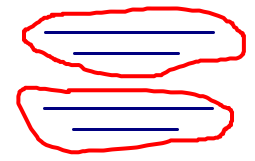
\includegraphics[height=2.5cm]{5+5}
\end{center}
Another student may have seen vertical lines of two, each shifted up or down from the previous.  So the schematic looks like this, with  the calculation  $2+2+2+2+2$:
\begin{center}

\includegraphics[height=2.5cm]{2+2+2+2+2}
\end{center}
Someone else might see diagonal lines and the calculation $4+3+2+1$:
\begin{center}

\includegraphics[height=2.5cm]{4+3+2+1}
\end{center}
Lots of variations on these ideas are possible, of course.  You might be surprised at how many different strategies your students will have for such a simple task. 

\item
Ask for a show of hands for students who thought about the problem in exactly the same way.  Then
ask if anyone else thought about it differently, and have one of those students share a different strategy.  Keep going until you have several different strategies to talk about.


\end{itemize}

Why spend time on an activity like these ``Math Talks''? Here are some answers to that question from teacher Cathy Humprheys.

\begin{quotation}
Cards with configurations of objects, that we often call ``dot'' card number talks, establish 
important new principles for mathematics classes. While it may seem that these arrangements of 
shapes are only for young children, we have found that they are critical for older students because they help to lay the groundwork for changing how students think 
about mathematics. Dot cards do not suggest procedures that students are ``supposed'' to follow; 
instead, they encourage students to think about what they ``see'' rather than what they are 
supposed to ``do.'' This frees up students for learning new ways of interacting in math class. 

Some of the things they can learn from dot card number talks:
\begin{itemize}
\item
Just as people ``see'' things differently, there are often many ways to approach any 
mathematical problem.
\item
 Explaining one�s thinking clearly is important. This requires that students retrace the 
steps of their answers and learn to use academic language, where possible, to describe 
what they did to solve the problem.
\item
It is important for students not only to explain what they did, but why their process makes 
sense. In the case of dot card number talks, this involves where they ``saw'' the numbers 
they used. In the case of arithmetic operations, it involves understanding the mathematics 
that underlies any procedure that they use.
\item
 The teacher's job is to ask questions that clarify what the students see rather than how 
they ``should'' see.
\end{itemize}
\end{quotation}

These are not activities to do every day, nor are they activities to occupy an entire class period.  Rather, these types of thinking, visualizing, and reasoning activities can be a great way to start or end class perhaps once a week during this session.  They tie very nicely to the ``dots and boxes'' representations of numbers.

You probably don't want to do too many of these number talks (you may use them more in the nedt session to practice computation).  But here are some other designs to try:

\begin{center}
\begin{tabular}{|cccc|}\hline
& & $\diamondsuit$ & $\diamondsuit$\\
$\diamondsuit$ &  $\diamondsuit$ &$\diamondsuit$ & $\diamondsuit$\\
$\diamondsuit$ &  $\diamondsuit$ &&\\
\hline
\end{tabular}

\bigskip

\begin{tabular}{|ccccc|}\hline
$\diamondsuit$ & $\diamondsuit$ && $\diamondsuit$& $\diamondsuit$\\
& &$\diamondsuit$ &  &\\
$\diamondsuit$ & $\diamondsuit$ && $\diamondsuit$& $\diamondsuit$\\
\hline
\end{tabular}

\bigskip

\begin{tabular}{|cccc|}\hline
$\diamondsuit$ & &   & \\
&$\diamondsuit$ &    & \\
$\diamondsuit$& &$\diamondsuit$ &\\
&$\diamondsuit$ &    &$\diamondsuit$ \\
$\diamondsuit$& &$\diamondsuit$  &\\
&$\diamondsuit$ &    & \\
$\diamondsuit$ & &   & \\
\hline
\end{tabular}

\end{center}




\subsection{Pitfalls and Additional Practice}
Most likely, your students will be fine with the mechanics of base 10 place value: writing numbers in expanded form, naming the place value for specific digits, saying what a digit is ``worth,'' and translating from written words to numerals.  If you find some or all of your students need to brush up on these skills, you can point them towards an online resource such as Kahn Academy\footnote{\url{https://www.khanacademy.org/math/arithmetic/multiplication-division/place_value/v/place-value-1}} or IXL\footnote{\url{http://www.ixl.com/math/place-values}}.  If you want to require them to complete such practice work, you can insist they email you a screen shot of completed worksheets or some other proof of completion.

More likely, students will make mistakes like mixing up ``power,'' ``multiple,'' and  ``factor'' (saying, for example, that in base 5 the positions are ``multiples of five'').   Correcting these mistakes requires reinforcement in class, gentle insistence or proper terminology in presentations and write-ups, and using problems targeting these issues.  (Some appear in the problem bank, and it is a simple matter to generate additional problems with a similar flavor.)


\subsection{Quizzes}
Here are some sample quiz questions that can be used with this chapter:

\begin{enumerate}
\item
For each problem, say if the equation is true or false.  Carefully justify your answer.

\begin{enumerate}
\item
$8_{\text{nine}} = 8_{\text{eleven}}$.


\item
$80_{\text{nine}} = 80_{\text{eleven}}$.
\end{enumerate}

\item
What number comes after $233_\text{four}$?  (Write your answer in base four.)

\item
Consider the number $122_b$, for some base $b$ that's bigger than 2.  Is that number even, no matter what base $b$ is?  Or is it possible for that number to be odd?  Justify your answer.

\item
Consider the number $222_b$, for some base $b$ that's bigger than 2. Is that number even, no matter what base $b$ is?  Or is it possible for that number to be odd?  Justify your answer.
\end{enumerate}


\newpage



\section{Chapter 3: Numbers and Operations}
The focus of this chapter is on encouraging students to think more deeply about what they ``know'' about addition, subtraction, multiplication, and division of whole numbers.  We use two models for thinking about the operations: 
\begin{itemize}
\item
We continue with James Tanton's ``Dots and Boxes'' model, which will allow us to explore the operations in bases other than ten.
\item
We introduce a measurement model, with a focus on the number line.

\end{itemize}

Note: The ``Dots and Boxes'' approach is essentially a set-theoretic development of the operations, without the formalism of sets, unions, intersections, and so on.  Some instructors like to introduce the formality of sets, explore these other binary operations, and include activities using Venn diagrams.  Such activities are not included in this chapter, but of course if you find these ideas appealing and engaging, you should take some class time out to explore them with your students.

One goal of this chapter is to get students in the mindset that elementary mathematics makes sense, and is not simply a set of rules to memorize.  We want to connect fundamental understanding of the operations --- addition is combining, subtraction is taking away, multiplication is repeated addition, and division is forming equal-sized groups --- with our models.  We then connect the models with the standard algorithms.  Finally, we use the models to explain some familiar facts like:
\begin{itemize}
\item
addition and multiplication are commutative and associative,
\item
multiplication distributes over addition, and
\item
division by 0 is undefined.
\end{itemize}
Often, our students know these facts procedurally --- they can use them appropriately in computations and perhaps even give the correct names.  However, they will say things like, ``Addition is commutative because $a+b=b+a$.'' They have no real understanding \emph{why} these arithmetic facts are true, or even that there is (and should be) an explanation for ``why.''   

The most important thing that students should get from the chapter is a clear understanding that they can always figure out ``why'' for some arithmetic fact.  They  should also know the difference between the definition of a property, some examples showing the property holds, and an actual explanation for why it is always true.  Explanations for only a couple of these arithmetic facts are actually presented in the student text, and students are asked to generate the others in the problems.  This is intentional.  These materials  provide a model for how to think about mathematics and how to figure things out, but are not meant to be an encyclopedic reference for elementary mathematics.

It is not essential that \emph{every} student  explains \emph{each} of the properties.  You may want to distribute the work amongst group, and perhaps take this opportunity to reprise activities where students look critically at each others' work after working on different problems (see the ``Writing Activity'' described in the Notes for Chapter~1).

The chapter consists of four sections and a ``Problem Bank.''

\begin{description}
\item[Model 1: Dots and Boxes]
This section develops the four operations --- addition as combining, subtraction as taking away, multiplication as repeated addition, and division as forming equal groups --- all in the context of the base 10 dots-and-boxes model.  (Some problems ask students to use the techniques in other bases, which will demonstrate a deeper understanding of the ideas, of course.)  Rather than jumping right into these activities, you may want to ask students to take their concepts of the operations from the chapter-launching Think/Pair/Share activity, and demonstrate what it looks like in the dots-and-boxes context, giving specific problems for them to demonstrate.  Students will probably easily demonstrate addition, but they often have trouble with subtraction.  They may line up the two numbers as they would for addition, and are then unsure what to do from there.  If some students work out a reasonable approach to subtraction, you can have them demonstrate it for the whole class, explicitly making the connection between subtraction and the action of taking away.  Alternately, students can read the  materials to see a more coherent development and to get common language moving forward.  Note that this section connects standard algorithms for addition, subtraction, and division to the model.  We work with the standard algorithm for multiplication in the next section.

\item[Model 2: Measurement]
This section introduces the idea of a basic unit and a measurement model for the operations based on assigning that unit the value one.  This idea comes back in the next chapter (``Fractions'').  That is previewed a bit in the launch activity, but you don't need spend a lot of time on fractions at this point.  Most of the section takes place on a number line.    We also introduce an area model for multiplication and connect it to the standard algorithm.  The distributive law is, of course, hiding just beneath the surface here.  Someone may mention this in class, but if not do not force it.  The formal properties of operations are discussed explicitly in the next section.  Two optional problems presenting non-standard multiplication algorithms close out the section.  These could be optional extra credit or the basis for an activity where different groups make sense of an algorithm and then teach the method to the class (including demonstrating examples and explaining why it works).




\item[Operations]
This rather lengthy section explores both the connections between operations --- subtraction as ``missing addend'' addition problems and division as ``missing factor'' multiplication problems --- and standard properties of the operations.  The emphasis throughout should be on finding ways to \emph{explain} these properties using our models.  In an IBL class, students will come up with their own explanations, which will be refined and polished through questioning by you and by the rest of the class.  (This may be a good time to divvy up work, asking different groups to focus on different properties and then presenting their work to the class.)  Alternately, you may want to present these explanations as a short lecture, or you may ask students to read the examples in the book.      Division is always the most difficult of the operations for elementary students (and teachers!) to master.  The section ends with a more lengthy discussion of the operation.
 If you have all students work through all of the problems, this section may start to feel repetitive, and it may be a bit of a slog  for some classes.   You may  want to break it up with a day of problem solving using problems from Chapter~1.  

\item[Division Explorations]
This optional section extends the dots-and-boxes division method to both base 5 and base $x$.  This gives students a chance to connect long division with the polynomial long division they likely learned in high school, perhaps making more sense of the latter.  Additionally, the problems suggest the idea of algebra as abstracting properties of \emph{operations}, and that true algebraic statements are true for any substitution of the variables.  Again, this section is optional, but we encourage you to give your students the opportunity to dig into  one of these optional sections at some point during the course.

\item[Problem Bank]
As usual, the problem bank contains potential homework and extra problems for use in class.  Pick and choose those that appeal to you.

\end{description}




\subsection{In Class Activities} 
There is not much in the way of ``practice of basic facts'' in the student chapter.  Remember that we assume students have some basic facility with computation, and we are trying to get them to think more deeply about the ideas in elementary mathematics.  

However, one of the main tasks for elementary teachers is develop number sense and flexible ideas about computation in their students.  Recent research by Eddie Gray and David Tall\footnote{\url{http://homepages.warwick.ac.uk/staff/David.Tall/pdfs/dot1991h-gray-procept-pme.pdf}} shows that students identified as high achieving by their teachers use more number sense in performing computational tasks, as opposed to memorization of facts or counting strategies.  In order to develop this number sense in their students, teachers certainly must have it themselves.

We provide here some in-class activities that may help students develop and reinforce their number sense.  Depending on the needs of your students, you may choose to do activities like these more or less often.


\subsubsection{Math talks}
Regular ``Number Math Talks''  provide one strategy for bringing number sense and computational practice into the classroom without making the chapter \emph{about } computation  facility.  (See the notes above on Chapter 2 for a similar version of this activity.)  Activities like this allow students to practice both computing  and articulating their strategies.  Having students share their strategies will allow everyone to grow their bank of strategies and their number sense.   But the focus in this case is squarely on the number sense and reasoning, rather than on speed and accuracy in computation.


 A Number Math Talk\footnote{For more on number talks, see \url{http://www.mathperspectives.com/num_talks.html}.}
 proceeds in this way:

\begin{itemize}
\item
Give students directions: They are to solve the arithmetic problem without writing anything down, and without using any standard algorithms.  When they have the answer, they are to simply give you a subtle ``thumbs up'' signal.  (Don't ask them to raise their hands.  This can be intimidating for students who work more slowly, if they notice lots of hands are up around them.  They can simply hold a thumb up close to their chest.)

\item
Pose an arithmetic question like $18 \times 5$, and wait until all students are giving you the thumbs up.

\item
Call on a student (this is a good time to randomly pull a name from the class list) to explain their answer.  Even if the answer is wrong, your response should be ``tell us how you got that,'' and ask the class to critique the method.  Usually students will self-correct as they explain, or someone in class can help them see an error.

\item
Ask for a show of hands for students who thought about the problem in exactly the same way.  Then
ask if anyone else thought about it differently, and have one of those students share a different strategy.  Keep going until you have several different strategies to talk about.

\item
Give a visual representation for each strategy presented.  For example, in $18 \times 5$, some students might compute $10 \times 5$ and $8 \times 5$ and then add.  So you might draw this picture:
\begin{center}
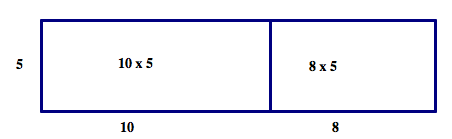
\includegraphics[height=2.5cm]{mult1}
\end{center}
Other students might use a double-and-half strategy like this: $18 \times 5 = 9 \times 10$.  So you might draw this picture.
\begin{center}
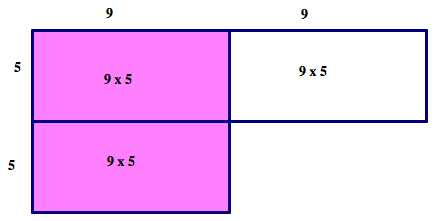
\includegraphics[height=4.5cm]{mult2}
\end{center}
Another student might compute $20 \times 5$ and subtract $2 \times 5$, leading to a picture like this one.
\begin{center}
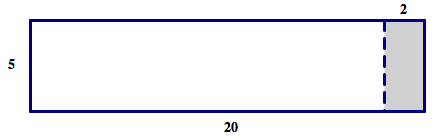
\includegraphics[height=2.5cm]{mult3}
\end{center}

\item
You can use the strategies and pictures to talk about what properties of arithmetic are being used: associativity?  distributive law? commutativity? others?

\item
If you'd like to spend more time on these strategies, you can present follow-up computations, even asking students to use a particular strategy this time.  (``See if you can use Tania's method on this computation.'')

\end{itemize}

You may wish to start one class per week with a Math Talk, or you may want to do them every day if you find your students need additional practice.  You may want to start with one  digit and two digit examples, then expand the activity to some well-chosen larger numbers.  Here are some suggested problems for each of the operations, with varying levels of difficulty.  
You can easily come up with many computations that lend themselves to this activity, using any of the four basic operations.  

\begin{center}
\begin{tabular}{cccc}
addition & subtraction & multiplication & division\\
\hline\hline
$7+18$ &$16-13$ & $8\times 9\times 3$ & $252 \div 4$\\
$27+52$ &$56-29$ & $4 \times 37$& $1710 \div 9$ \\
$342+561+52$  & $751-647$& $37 \times 98$& $1225 \div 25$ \\
$198+387$ & $83-37$& $4\times 13\times 25$& $72 \div 12$\\
$32 + 29 + 56$ & $214-86$ & $26\times 24 - 21\times 24$& $120 \div 15$ \\
$54 + 28 + 67$ &$52-35$ &$84\times 5$ & $145 \div 5$\\
$49 + 252$ & $173-96$& $37 \times 99$ & 
\end{tabular}
\end{center}


\subsubsection{Four 4's}
The four 4's game works this way: Challenge students (individually or in groups) to make every number from 1--20 using just four 4's (as digits) and basic operations.  For example, you can make the number 1 in several ways:
$1 = 44 \div 44$,  $1 = (4 \div 4)^{44}$,  $1 = (4 \div 4) + (4-4)$, and so on.

To complete some of the challenges, students may need to go beyond the four operations in this chapter, using square roots, exponents, and maybe even factorials.  You can take the opportunity of having them share their answers to discuss the meanings of these functions.  

The activity may also lead to a conversation about order of operations, though it is not an explicit part of these materials since it is not in the K--5 for the Common Core State Standards.  Like the other functions mentioned, order of operations should be familiar to students, and it's fine to take some time to discuss it when it comes up naturally in an activity.

You can play the same game with other digits.  For example, you might use the digits of a year.  On President Obama's birthday, you can play the activity with his birth year of 1961.



\subsubsection{24}
This is a card game similar to the ``Four 4's'' game above.  In groups of three or four, each group is given a deck of cards.  (You may choose to remove face cards, assign them values, treat them all as ten, or whatever.)  Someone deals out four cards face up.  The goal is to use the four cards and any arithmetic operations / functions to create the number 24.  For example, if the group is dealt a 3, 4, 5, and 10 you could write: $10 \cdot(5-3) + 4 = 24$.  

Whoever can form 24 first gets a point, and when all the cards have been used the person with the most points wins.  If a group thinks making 24 is impossible with the four cards that have been dealt, they can agree to re-shuffle and deal four new cards.  Or you may ask that they check with you, and if you see a way to make 24, encourage them to keep trying because it is possible.



\subsection{Materials}
At the end of Section 1, if you have base-10 blocks available, you may want to ask students to demonstrate the same calculations they have done with dots-and-boxes using those materials and physically regrouping.  Make note for them that the base 10 materials (common in elementary schools) allow them to get at many of the same ideas about standard algorithms.  However, they force you to work in base 10 whereas the dots and boxes approach is more flexible. 

In the introduction to Section 2, if you have access to the materials to do so, you  might wish to include a short activity on using volume to model operations in a measurement model as well.  
This would require some containers with various sizes / shapes or with markings at different levels so that one of the containers (or markings) can be measured off in terms of the other one.  (Colored water is particularly nice to use for these demonstrations, since it's more visible.) 

Ask students to demonstrate adding and subtracting using the containers.  For multiplying, note that you can multiply some volume by a number, but you can't multiply two volumes.  You can, however, divide one volume by another.  Ask students to demonstrate what that would mean.

Also in Section 2, we encourage you to actually get students up and moving in this activity.  If you can, take them outside and draw number lines in sidewalk chalk.  Have them physically solve the problems with a partner, taking turns pacing out the answers.  They need to internalize ``subtraction means walk backwards,'' as well as how to do the division algorithm by keeping track of how many times they move forward. 

If you opt to discuss negative numbers with your class, extending this model allows students to explain, for example, why subtracting a negative number and adding a positive number have the same effect: face negative and walk backwards (subtract a negative) is the same as face positive and walk forwards (add a positive).  Similar explanations allow students to explain familiar rules like ``negative times negative equals positive.''


\subsection{Quizzes}
Some options for quizzes: 
\begin{itemize}
\item
Ask students to use both models to demonstrate a simple calculation.
\item
After an arithmetic fact has been discussed in class, ask students to explain why it is true on a quiz.  
\item
As an exit ticket,  ask students to generate  a good quiz question.  Then pick one of two of these student-generated questions to use on a quiz during the next class.  
\item
Some of the ``Problem Bank'' problems are reasonable quiz questions.  
\end{itemize}  



\newpage

\section{Chapter 4: Fractions}
The topic of fractions is one of the hardest  to teach and learn in elementary school, and it is the one area where Math 111 and 112 students are consistently weak in both skills and conceptual understanding.  

We address this issue directly, with three sections on the subject of ``What is a fraction?'' in which we unpack some of the difficulty that K--5 students have with these ideas, and where that difficulty comes from.

As in the ``Number and Operations'' chapter, we focus on understanding different models for fractions, using those models to make sense of operations, and focusing on why the algorithms for computing with fractions make sense.

We also work on developing some fraction number sense.   Throughout this chapter, you should discourage students from using decimal equivalents.  Remind them that elementary students learn about fractions first, and they will need to teach fraction ideas without resorting to decimal representations.  You should discourage the use of calculators.  If students offer problem solutions or justifications based on decimal representations,  ask students if they can also work it out another way.

Much of the material in this chapter was adapted from James Tanton's ``Guide to Everything Fractions,'' which you can find in its entirety on his website.\footnote{\url{http://www.jamestanton.com/wp-content/uploads/2009/07/fractions-guide.pdf}}

The chapter consists of nine sections, a Problem Bank, and two optional extensions.  This chapter, in particular, lends itself to many in-class activities that are not written up in the student text.  See later in these notes for ideas for these activities.

\begin{description}
\item[What is a Fraction?]
We introduce our first model for fractions: a fraction is the answer to a division problem.  We call this the ``Pies Per Boy'' model.  That is, the fraction $\frac a b$ represents the answer to the division problem $a \div b$, and the answer to the question ``If $a$ boys share $b$ pies, and everyone gets the same amount, how much pie does each individual boy get?''  Students are asked to explore the model and think about questions like what $\frac a a$ means and what it might mean to divide by $\frac 1 2$.  All of these topics will be revisited later, so there's no need to delve into them too deeply at this point.  

\item[The Key Fraction Rule]
This section tackles equivalent fractions and uses the ``Pies Per Boy'' model to explain why it is true that $\frac{xa}{xb} = \frac a b$, at least for positive whole numbers $x$.  Right now, we are looking for intuitive understanding.  We will provide a more rigorous proof of the equivalence in a later section.

\item[Adding and Subtracting Fractions]
This section develops the algorithms for adding and subtracting fractions with like and then unlike denominators.  The method presented is via equivalent fractions, in order to reinforce our ``key fraction rule.''  Some students may recall that they ``should'' use the LCM of the denominators (or they may incorrectly remember that they ``should'' use the GCF of the denominators) when adding and subtracting.  Since LCM and GCF are not part of the K--5 curriculum in the Common Core State Standards, these topics are not covered in depth in our Math 111 and 112 courses.  As the instructor, you should decide how much to pursue these ideas should they arise in your class.  It is important to keep the focus on sense-making: In fact, it doesn't matter \emph{which} common denominator we use.  Any one will do!  We could just as easily say that we ``should'' use the  product of the denominators since it always works and doesn't require the additional LCM computation.  If these ideas come up in class, you might pose a question to students: why do they think elementary students are taught to use the LCM as a common denominator?  What are the benefits of that choice versus another choice you might make?

\item[What is a Fraction? Revisited]
This section expands our fraction model to be simply ``parts of some whole,'' discussing units and unitizing.  The motivation here is that if we wish to move on to multiplying and dividing fractions (and certainly we do!), then the ``Pies Per Boy'' model is no longer adequate because we don't have a way of making sense of multiplication in that model.  This section also discusses ordering fractions, and  arithmetic sequences are introduced.  Students are challenged to form arithmetic sequences of fractions with  given starting and ending values.  These problems can be  challenging, but we encourage you to let students struggle and make sense of them rather than providing canned methods for solving them.

\item[Multiplying Fractions]
Given the number line model for fractions, we are able to return to the area model for multiplication used in the ``Number and Operations'' chapter.  Using this model, we develop the standard ``multiply the numerators and multiply the denominators'' procedure for fraction multiplication.  Tying that procedure back to the picture lets students understand why it makes sense in terms of ``parts of a whole.''  The complication here is that the factors are parts of \emph{segments} and the product is part of a \emph{square}.  This shift in dimension may be confusing to students, but point out that it is no different than the whole number case.  Even there, the sides are numbers of unit lengths, and the product is a number of unit squares.  The section ends with a careful justification of our ``key fraction rule'' based on thinking about multiplication by 1.

\item[Dividing Fractions: Meaning]
This section revisits the partitive, quotative, and missing factor models of division where the numbers in question are fractions.  The focus is on making sense of the problems and drawing pictures to represent the situations.  Computational methods are discussed in the next section.


\item[Dividing Fractions: Computations]
This section provides several ways to think about computing division of fractions problems.  We start with ``if the fractions have the same denominator, then just divide the numerators,'' and use that to develop a common denominator method for division.  We also use a missing factor approach, but it is clearly limited in its utility based on the fractions in the problem.  This method is particularly satisfying because it makes sense to students.  Our goal is to move away from the mindless, ``ours is not to reason why\dots\ just invert and multiply'' philosophy that most students have about these problems.  We then introduce division of fractions by ``simplifying an ugly fraction'' (one where the numerator and denominators are themselves fractions or mixed numbers).  This leads finally to a justification for the ``invert the second fraction and multiply'' method.  Finally, we ask students to compare the four methods for dividing fractions and discuss the pros and cons of each.

\item[Fraction Sense]
In this section, students think about how the size of (positive) numbers change when the four basic operation are performed.   Because of the symbols, the opening problem may look quite intimidating to students.  You might want to pose just the first line (addition) and see what they can do with it.  The goal is to get students to invent lots of examples to test out in order to make a decision, and then to use those examples to help them craft an explanation.   The section ends by revisiting the question of division by zero, this time in the context of fractions $\frac 0 a$ and $\frac b 0$.

\item[Problem Bank]
There are lots of problems here, again too many to assign or use all of them.  In addition, if you spend time in class on some of the activities described below, you may assign more of the readings, exercises, and problems from the other sections for homework.  Draw on these problems as you see fit.

\item[Egyptian Fractions]
This optional section explores the idea of Egyptian fractions.  You may choose to spend time in class on the subject (providing extra practice with addition, subtraction, and problem solving with fractions).  Alternately, you may want to offer this section as an optional extra credit activity for interested students.

\item[Algebra Connections]
For students with a stronger background, this section gets them to simplify seemingly complicated algebraic expressions using the techniques of this chapter.  The goal is to reinforce the idea of algebra as ``generalized arithmetic''.

\item[What is a Fraction? Part 3]
This final section revisits for a third time the reason that fractions can be so difficult a topic for elementary teachers and students.  We present a bit of the mathematical formalism of fractions as equivalence classes of whole numbers.  Finally, we ask students to think about what they've learned and discuss how they like to think about fractions, now that the chapter is complete.

\end{description}

\subsection*{In Class Activities}
This chapter, perhaps more than the others, lends itself to many in-class activities that don't necessarily translate well to a student text.  We describe several such activities here.  These are all, of course, optional.  The idea is to provide lots of examples of the kinds of activities that might engage students and reinforce the ideas in the chapter.

\subsubsection*{Math talks}
You may wish to adapt the ``Math Talks'' described in Chapters 2 and 3 to include simple fraction computations, especially if you feel your students need additional computation practice.  The talks can be adapted to include questions like ``Is this sum more or less than $\frac 1 2$?: $\frac 1 3 + \frac 1 4$'' or ``Is the answer to $1 \div \frac 2{3}$ more or less than 1?  (Answer without computing.)''   or ``Estimate $\frac 7 8  + \frac{11}{13}$ without computing it.  Which number is it closest to and why? 1, 2, 19, or 20?''



\subsubsection*{Fracitons in-between}
Draw a long number line on the board,  with zero on one end and one on the other.  Ask someone: put a fraction about where it belongs on the board.  Continue until everyone has placed a fraction.
If necessary, repeat with rule that students have to put a fraction between two that were placed by other students (to avoid sequences like $\frac 1 2$, $\frac 1 3$, $\frac 1 4$, \dots\

You can debrief the activity with a discussion:  How many fractions are there  between 0 and 1?   Why?  How many fractions between any two fractions?  How to find a fraction between any two that are given?

\subsubsection*{Justification of ``sometimes true''}
We find that ``always / sometimes / never true?'' questions are useful for quick assessments at the end of class.  For example is the following statement always true, sometimes true or never true?

\begin{center}
\emph{The greater the numerator, the greater the fraction.}
\end{center}

Students often have a difficult time justifying that statements are ``sometimes true.''  
Some students may correctly answer ``sometimes true,'' but may not realize that to justify that answer they must show \emph{both} an example where it is true and an example where it is false.  You can pose the question to students, ask them to come up with a good justification, and then have several groups share their justifications. 




\subsubsection*{Multiplication and Division}
For each of the following expressions, ask students to write a word problem.  Then they should solve their own problems (or exchange problems with a partner or another group and solve each others' problems).
\[
 3 \times \frac 1 2
\qquad\qquad
 \div \frac 1 2
\qquad\qquad
\frac 1 3 \times 4
\qquad\qquad
\frac 1 3 \div 4
\qquad\qquad
\frac 5 8  \times \frac 1 4 
\qquad\qquad
\frac 5 8 \div \frac 1 4
\]

You can, of course, collect these problems and pull a few of them to use as questions on a future quiz.


\subsubsection*{Rational tangles} Conway's rational tangles activity is described in detail here: \url{http://www.geometer.org/mathcircles/tangle.pdf}\footnote{You can view a (long) video of the activity run with teachers here: \url{http://www.youtube.com/watch?v=iE38AXV_dHc}.}.  It's an engaging class that deals with creating a mathematical model of a fun situation along with practice computing with fractions.  It's quite satisfying to students when they compute the answer and then it works out, the knot actually unties!

\subsubsection*{Fraction war}
Students can play fraction war with cards.
You might want to start by having someone explain the rules to the card game ``War.''  Then describe this  modified version:


In pairs or threess: Shuffle cards well, then  split the deck of cards evenly between the players.  (They will need to leave out a single card if there are three players.  You can designate a card to be left out, like the ace of spades.)

Each person turns over the top two cards in their hand and forms a fraction by putting low number / high number.  The person with the largest fraction wins.  (Students  need to agree on which is bigger\dots\ no calculators!)  
The winner takes all four (or six) cards and puts them face up below his cards.  

As with War, if there's a tie the cards stay out and there is another round of play.  The winner of the second round takes all cards from both rounds.  (Repeat as many times as necessary until there is no longer a tie.)

When all cards have been played (players get to face up cards), the winner is the one with the most cards in her deck.

Variations: Smallest fraction wins. Put high number / low number and smaller (or larger) wins.  Put low / high and fraction closest to $\frac 1 2$ wins.


\subsection*{Quiz and test questions}
You can, of course, draw problems from the ``Problem Bank'' for quizzes, or use questions that students generate in class activities like those described above.  Here are some other questions you might want to use.


\begin{itemize}
\item
Your student asks if you can draw a picture to explain what $\displaystyle \frac 3 4$ of $\displaystyle \frac 5 7$ means.  What would you draw?

\item
Explain how each of the following fractions could be represented by the drawing below.
\[
\frac 7 8 
\qquad \qquad\qquad
3\frac 1 2
\qquad \qquad\qquad
1 \frac 3 4
\]
\begin{center}
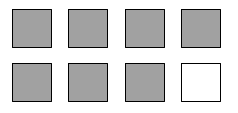
\includegraphics[height=4cm]{DiffFracs}
\end{center}



\item
Lynne calculates
\[
\frac 3 4 \div \frac1 4 = 3.
\]
Then she says, ``I don't get it!  The answer is bigger than both $\displaystyle \frac 3 4 $ and $\displaystyle \frac1 4$.  How can that be?''


\begin{enumerate}[(a)]
\item
Did Lynne calculate correctly, or did she make a mistake?  Explain how you know.

\item
How would you help answer Lynne's question?

\end{enumerate}


\item
Here is an unordered list of fractions.  Answer the following questions using benchmarks and other intuitive methods.  {\bf Do not use decimals, and do not use a common denominator.}


\[
  \frac{3}{2}, \qquad\frac{7}{8}, \qquad\frac{4}{5}, \qquad \frac{1}{6}, \qquad\frac{3}{4}, \qquad\frac{1}{3}, \qquad\frac{3}{5}, \qquad\frac{5}{11},\qquad \frac{9}{8}, \qquad\frac{1}{4}, \qquad \frac{1}{10}.
\]


\begin{enumerate}[(a)]
\item
List all of the fractions given above that are greater than~$1$.  Explain how you know the fractions are greater than~$1$.

\item
List all of the fractions given above that are greater than~$\frac 1 2$ but less than~$1$.  Explain your answer.


\item
List all of the fractions given above that are less than~$\frac 1 2$.  Explain how you know the fractions are less than~$\frac 1 2$.


\item
Put the whole list of fractions in order, from smallest to largest.  You do not have to explain your work.

\vspace{.5in}

\end{enumerate}


\item
For each pair of fractions, decide which is larger.  Circle your choice and {\bf justify} it.  
\bigskip

\[
\frac{997 }{ 999} \qquad   \text{  or }  \qquad  \frac{99997}{99999}
\]




\[
\frac{15 }{ 337}  \qquad \text{  or }  \qquad  \frac{15}{773}
\]


\item
Write the missing-factor multiplication problem for this division problem.  Then use what you know about multiplication of fractions to solve the problem.  Show your work clearly.  (Do not draw an area model!)

\[
\frac{5}{12} \div \frac{1}{3}= \underline{\quad \phantom{\frac{5}{4}}\quad }.
\]

\item
Solve this division problem with the common denominator method.  Show your work clearly.  
\[
\frac{3}{4} \div \frac{1}{12}= \underline{\quad \phantom{\frac{5}{12}}\quad }.
\]


\item
Draw an area model to show $\displaystyle \frac 2 3 \times \frac 3 5$ and then find the answer.



\item
For each problem circle either TRUE or FALSE.  Provide a clear justification of your choice.  (Don't just state a ``rule','' but explain \emph{why} your choice is correct.)


\begin{enumerate}[(a)]
\item
$\displaystyle \frac 5 7 + \frac 3 8 = \frac 8{15}$.
\begin{center}
TRUE \qquad \qquad  FALSE
\end{center}

\item
The quotient $\displaystyle \frac6{11}\div \frac7{13}$ is the same as the product $\displaystyle \frac{11}6 \cdot \frac7{13}$.
\bigskip

\begin{center}
TRUE \qquad \qquad  FALSE
\end{center}
\item
There is a fraction between $\displaystyle\frac 3{29} $ and  $\displaystyle\frac 4{29} $.

\begin{center}
TRUE \qquad \qquad  FALSE
\end{center}
\vfill
\end{enumerate}


\item
Solve each of these problems.  Think carefully about what answer makes sense.  Drawing a picture might help!


\begin{enumerate}[(a)]
\item
Inga was making a cake that called for $2\frac{2}{3}$ cups of flour.  But the only clean measuring cup was  $\frac 1 3$ cup.  How many scoops of flour with the $\frac 1 3$ cup will she need to make the recipe?


\item
After his birthday party, John had $2\frac{2}{3}$  pizzas left over.  John  ate $\frac{1}{3}$ of the leftover pizza.  How much pizza did John eat?
\vfill
\end{enumerate}

\item
Determine which of the following are correct or incorrect.  {\bf Justify your answer.}

\begin{enumerate}
\item
$\displaystyle
\frac{a\cdot\cancel{b} + c\cdot\cancel{b}}{\cancel{b}} = a+c$.




\item
$\displaystyle
\frac{\cancel{a} + b}{\cancel{a} + c} =\frac b c$.


\end{enumerate}

\item
Jim gave a fourth of the money in his pocket to Tom. Then, he gave a third of what was left to Zoe. Then he split the remainder with you. If Jim gave you \$20, how much money did he have before he started giving it away?




\item
The points are evenly spaced on the number line.  What fraction corresponds to point~$E$?

\begin{center}
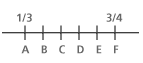
\includegraphics[height=2cm]{ArithSeq}
\end{center}



\item
Draw an area model to show $\frac 3 4 \times \frac 2 5$ and then find the answer.



\item
Draw a picture to illustrate this situation; use your picture to answer the questions:  There was $\frac 2 3$ of a pie leftover in the fridge.  John ate $\frac 2 3$ of that leftover pie.  


\begin{enumerate}
\item
How much of the pie did John eat?  Justify your answer.

\item
How much of the pie was left when he was done?  Justify your answer.

\end{enumerate}



\item
Draw a picture of the following problem, and then use your picture to solve it.


\begin{quotation}
\emph{Jeanette wants to tie pieces of ribbon around bags of cookies that she'll sell at a fundraiser.  She wants to cut each piece of ribbon to be exactly $\frac 2 3$ of an inch long.  Her original ribbon is $6$ inches long.  How many pieces can she cut?}
\end{quotation}


\end{itemize}



Four chapters make up the Math 112 course materials:
\begin{enumerate}
\item
Patterns and Algebraic Thinking (4--5 weeks)
\item
Place Value and Decimals (about 5 weeks)
\item
Geometry (about 4 weeks)
\item
Navigation on H\=ok\=ule\kern.05em`\kern.05em\relax a (about 2 weeks)
\end{enumerate}
(Note: number of days and weeks in these notes is for a MWF schedule.  Alter for a TR schedule as appropriate.)


You will probably  alter these suggested timelines as it suits your style and the needs of your class. 
If you feel students are struggling or just not getting one particular topic, it may not be fruitful to stick with it and insist on mastery by the whole class.  Remember that we are trying to provide students with the tools to \emph{eventually} develop profound understanding of fundamental mathematics, but we do not believe we can get them there in a semester or a year.  Use your professional judgment about when it is worth spending more time, when  to move on, and when to skip sections entirely.

The materials include readings for the students, activities for in-class use, and problem banks.  Some chapters will include suggestions for self-checks on procedural skills, since these are assumed as background knowledge.  As an instructor, you may wish to require that students submit to you proof of passing such assessments, or you may want to supplement the materials with some skills practice if you deem it necessary for the majority of your students.


A typical class might proceed as follows:
\begin{itemize}
\item
Whole-class discussion about a homework problem or  reading.  To start the discussion,  a student  presents her solution to the problem or summarizes what was discussed in the reading.
\item
Think/pair/share\footnote{This is a standard methodology used in inquiry-based learning.  Read a description here: \url{http://theiblblog.blogspot.com/2011/08/classroom-strategy-think-pair-share.html}.} for a launch activity.   These are labeled in the materials under this heading.
\item
Call on individuals or groups to present their work.  Depending on the activity, there may be just one presentation or more than one.  (You may want to give the groups a few minutes notice so they can prepare what to say.)  Emphasize that these presentations are launch points for a class discussion, so students are not expected to give polished solutions after a partial class period.
\item
Debrief the launch activity.  This may include student presentations or a short instructor   lecture on key ideas.  (In an IBL class, the content marked ``Definition'' or ``Example'' in the student materials should grow out of student work on the ``Think / pair / share'' activities and the problems rather than assigned as readings during class.   Including these materials in the text is intended to give students a reference for later study.  Working on and presenting problems, not reading the text, should be the main activity during class time.)
\item
The rest of class will vary depending on the activity and the class: Students may continue working on the problem with the expectation of finishing a good write-up by the end of class or for homework.  There may be a short quiz or other individual assessment.  Students may read from the course materials and then work on a problem or  another Think/pair/share activity. 
\end{itemize}

For most Math 112 classes, there will be a lot of group work both in and out of class.  Students will often collaborate on their homework, though instructors should insist that write-ups are individual work except on assignments that are explicitly assigned to groups.    Weaker students may be inclined to defer to group members rather than assert themselves to ask questions and make sure they follow along. 

 As an instructor, you can look out for these situations as the groups are working, check in with individual students, and help the groups take responsibility for all members' understanding.  (One method: call randomly on students to present and assign a score to the group based on the quality of that presentation.  It is therefore in the group's best interest to insure that everyone participates and understands the solution.)

In addition to helping the groups as they work, it is useful to have regular individual assessments.  Quizzes and  ``exit tickets''\footnote{Usually this is a short, often anonymous, questionnaire done at the end of class that students must turn in before leaving.  Typical questions: ``One thing I understand from today's class is \underline{
\qquad\qquad\qquad}.  One thing I do not understand well is \underline{
\qquad\qquad\qquad}.  One question or concern I have is \underline{
\qquad\qquad\qquad}.''   You can read other ideas here: \url{http://www.adlit.org/strategies/19805/}.}  can help you identify students who are struggling and help these students see for themselves how they are doing.


\subsection*{Choice of content}
The content for Math 111 / 112 was selected to align with the Common Core State Standards\footnote{\url{http://www.corestandards.org/Math}} for grades K--5.  Some content that appears in many ``Math for Elementary Teachers'' textbooks is not included in these materials, because it does not appear in the K--5 curriculum.  This includes:
\begin{itemize}
\item 
Integers (negative numbers)
\item
Ratio and proportion
\item
Prime factorization, gcf, and lcm
\end{itemize}

Our intent is to focus on depth of coverage for the K--5 curriculum and on the process of doing mathematics and justifying solutions, 
rather than rushing to cover many more topics.  

We encourage you to spend time in class letting students struggle and find their own way.  Ask questions rather than explaining.  Remember that your students will eventually have to make sense of mathematical ideas without your guidance.  They will have to become the mathematics experts in their own classrooms.  It is far more important that we affect their view of mathematics and of themselves as learners and doers of mathematics than that we cover any particular piece of the elementary curriculum.







\newpage

\section{Chapter 1:  Patterns and Algebraic Thinking}
Starting with the ``Patterns and Algebraic Thinking'' chapter allows you to set the tone for the class.  The message to students is intended to be:

\begin{itemize}
\item
Mathematics is about solving problems and explaining your work to others.
\item
You should always be able to explain \emph{why} your answer is correct for any mathematical problem (or exercise).
\end{itemize}

Another major theme is the different kinds of algebraic thinking.  Most students think of algebra in a very procedural ``solving for $x$'' kind of way.    For example,  Carolyn Kieran found that when students were asked to express the meaning of $a+3$, they couldn't because there is no equals sign and no number on the other side.

 The use of variables to express relationships rather than as ``unknowns'' where we solve an equation is really at the heart of algebra, and a much more useful skill for students.  As part of the Common Core State Standards, elementary teachers are expected to foster algebraic thinking (reasoning abstractly, using symbols, and using multiple representations) from very early grades.  It's important to emphasize the different kinds of algebraic thinking for future teachers, and to help them develop their own facility at structural algebraic thinking.
 
 A note on the use of variables:
 This chapter makes a concerted effort not to follow the ``convention'' (such as it is) of using the first letter of an object as a variable.  First, we want to develop in our students a more flexible use of variables and the realization that \emph{any} letter (or really any symbol) can be used to represent an unknown or a varying quantity.  More importantly, research by Jere Confrey indicates that it's actually confusing to students to follow this ``convention.''  For example, consider the question:
 
 \begin{quote}
 \emph{Apples are priced at \$1.00 each and oranges are priced at \$0.75 each.  What is the total cost of buying some number of apples and some other number of oranges?}
 \end{quote}
 
 We might be tempted to write as a solution:
 \[
 \$1.00 a + \$0.75 o
 \]
 where $a$ represents apples and $o$ represents oranges.  But of course this is silly!  We can't add apples to oranges.  In fact, in this expression, $a$ represents \emph{the number of apples purchased}; it does not represent apples.  So it would be more reasonable (and in fact more clear) to write something like
  \[
 \$1.00 n + \$0.75 m
 \]
 where $n$ represents some number of apples and $m$ represents some number of oranges.  
 
Mathematicians use this ``first letter' convention so often that we don't realize it, yet to students who struggle with algebraic notation, it is confusing.  They do, in fact, feel like they are adding ``apples to oranges,'' and have trouble making sense of the situation.

You may or may not want to make this choice clear to students, and you should certainly insist that students are very clear on their variable assignments: not apples, but some number of apples, and so on.


The chapter contains a short warm-up activity (probably best done during the first class after other class business), followed by five sections and a Problem Bank:

\subsection{Borders on a Square} 
Rather than working from the text, you may want do conduct this as an in-class ``math talk'' activity.\footnote{See Section 2.2 of the Math 111 Course Outline Instructor Notes for  more detailed descriptions of these ``math talks.''}     Briefly show and describe the first picture (a $10 \times 10$ square with red squares along the border) and explain the problem (figure out the number of red squares without counting one-by-one).  When students have an answer, they should give a subtle ``thumbs-up'' against their chest and wait for others to finish.  When all (or at least most) students are giving the thumbs up, ask several students to describe and justify their solutions.  

 On the board, you can write the solution along with a helpful picture or description like those in the book.   Name solutions after the students who propose them.  Be sure to keep asking, ``Did anyone figure it out a different way?''  
If not all of the calculations described in Problem 3 are suggested, you may then show students those computations (claiming them as your own method, perhaps) and ask students to create the justifications.  Then go on to the follow-up questions about varying the dimensions of the larger square.    

Problem 6 makes a good homework assignment for students to write up on their own.  The activity concludes with a ``Think / Pair / Share'' asking students to summarize and generalize what they have found.  After a class discussion on the ideas, those questions could also be used as writing prompts.  The entire activity is probably one or 1.5 class sessions.

\subsection{Careful Use of Language in Mathematics: =}
 In Math 111, students spent some time thinking about being precise with their language, the meaning of ``or,'' and how to interpret conditional statements.  This section continues that conversation with a focus on the symbol ``=''.   We want these future teachers to be precise in their use of the = sign, not using it (as we so often see) to carry out several steps in succession, and not using it to announce results.  Rather, they should see it as a symmetric relationship, indicating that two expressions separated by the = sign are equivalent, even though they make look different.  

One structure for moving through this section: Assign Problems 7--10 for homework. During the next class, have students check each others' work on the homework and provide feedback.  You may wish to collect the homework, or to allow students to revise it base on their partners' feedback before collecting it.    Then show the whole class Kim's proposed solution to Problem 7, and ask them to discuss it with their partner, pointing out both positive and negative aspects of the solution.  Follow up with first partners and then the whole class working on a good definition of the symbol = and a description of when and how it should (and should not) be used.  This could easily take an entire class period.   

The second class can launch with the first balance puzzle, with students working on the puzzle in small groups and then asking one or two groups to present their solutions and their reasoning.  Students will have different approaches, but you should emphasize the goal of maintaining a balanced scale throughout the process.  It will probably take at least two days of class time to have groups work through the balance scale puzzles and present their solutions.  You may decide to do fewer problems in class, assigning some for individual homework instead.  Or you may want to to assign the mobile problems from the Problem Bank (Problems 41 and 42) for homework after having done the balance scale problems in class. 




\subsection{Growing Patterns}
This section provides students with several sequences of figures made from colored tiles.  Students are asked to describe how the patterns grow and to use that growth to predict what will happen in future terms of the pattern.  

The launch activity involves the famous ``staircase problem.''   If possible, give students colored tiles with which they can build the next several terms of the sequence.   The first question for each pattern, and the one that should be the initial focus, is to describe ``How does this pattern grow?''  If you ask students to focus too early on the question of number of tiles in different figures, it encourages them to make tables and look for patterns in the tables, losing the context of the visual pattern.  The ultimate goal is, indeed,  to have some kind of formula (either closed-form or recursive) to describe the number of tiles used to build each term in the sequence.  However, it's essential that students can justify their formulas based on how the patterns are growing, rather than just focusing on sequences of numbers.\footnote{If students are too eager to focus on numerical patterns and resist providing justifications based on the pictures, you may want to revisit the ``Beware of Patterns!'' activity from Module 1: Problem Solving from Math 111.  This activity presents an ``obvious'' numerical pattern that breaks down after the first few steps.}

Since this problem  has a quadratic growth pattern, it is unlikely that students will come up with a closed form for the number of tiles in each term of this sequence, and that is not really the goal.  Rather, you want to encourage them to be clear --- using words, pictures, and variables --- in answering the question ``How does this pattern grow?''  Several examples of using pictures to describe the growth are presented in the text, but even better would be to pull examples from your own students' approaches.  The goal of the launch activity is that students have several models for describing the growth of a visual pattern like this before tackling several problems on their own.  In answer to the question ``How can you compute the number of tiles in any figure in the pattern?'' it is likely that students will respond with a formula like $1+2+3+\cdots +n$ where $n$ is the figure number.

Problem 15 provides some visual clues to lead students towards a closed form rule for the staircase pattern.  It could be considered an optional problem, to be covered if you have time or if your students are still engaged in the question.  There is no discussion in the text about the difference between closed-form and recursive rules, so if you cover Problem 15, you may want to bring up this idea in class so that students have a way to articulate the difference.


Following the launch, students are presented with several more growing patterns to explore and describe.  There are many possible approaches.  You may opt to split the class into groups and give one pattern to each group to explore, understand, and clearly present to the rest of the class.  Or you may want to take more time, having each of the groups work with at least most of the patterns.

Depending on how you structure the section, you will likely spend three to five class periods on these activities.  Problems 37--40 provide similar questions around visual patterns made with toothpicks.  They would make reasonable homework questions during this week of class, or a quiz question at the end of the activity.





\subsection{Matching Game}\label{subsec: matching}
In mathematics education, there is a so-called ``rule of four,'' meaning students should be able to represent mathematical objects in multiple ways.  For example, they should be able to represent functions with graphs, tables, equations, and words.  Hopefully, students have already been using at least of few of these representations in their explanations of the growing patterns in the previous section.  This activity simply makes these multiple representations more explicit.  Students are asked to match visual patterns, input / output tables, equations, and descriptions in words.

This is intended to be done as an in-class activity, taking a single class period.  One way to run this activity is to copy the objects onto colored notecards, for example blue for the equations, red for the patterns, yellow for the descriptions in words, and so on.

Pass out the visual patterns to each group, and ask them to arrange them in some way that makes sense to them.  When most of the groups have completed that task, pass out the cards containing the equations and ask the same question.  Follow with the tables of numbers, and finally the descriptions in words.  Students should realize the connections between the different representations on their own, and should start organizing them into ``stacks'' of objects that correspond.  

 
Conclude with a whole-class discussion of what they noticed, a few specific examples of multiple representations with justifications, and some remarks about potentially strange cases (like when you have multiple formulas that match the same visual pattern).  You can make the ``rule of 4'' explicit, and encourage them to think about multiple ways to describe mathematical ideas as they work.

Potential homework problems would be to provide the other three representations for the visual patterns give in Problems 37--40 of the Problem Bank.




\subsection{Structural and Procedural Algebra}
This last section makes the distinction between structural and procedural algebra explicit for your students.  You may want to launch the activity with the ``Think / Pair / Share,'' with a whole-class discussion of their ideas.  You can then ask students to read the description on the first page of the activity.  If their school math was overly focused on procedural algebra skills, they likely had trouble with the   ``$a+3$'' question, and they are not alone.  But emphasize that this kind of descriptive use of algebra is what's really useful in life.  (For example, many people will be asked to program a simple spreadsheet to make some calculations, but few people will be asked to solve very complicated equations by hand.  Actually setting up the equations and knowing what they represent is a far more useful skill in our modern age.)


Following the launch, you will probably have four or five days of class on this activity.  First, students can work individually or in groups on Problems 21--23, connecting algebraic equations to situations.  During the second class, groups of students might work on the balance scale activities (Problems 24--31), with some of their groups presenting their work on the third day of class.  Problem 32 could be done in class or for homework.

The first part of the section wraps up with a class discussion revisiting the concepts of structural and procedural algebra, and reflecting on the mathematical thinking they did in these problems.

The subsection on ``variables and equations'' makes explicit that not only do we view variables in different ways given the context (either an unknown to be solved for or a varying quantity), but the same is true of equations.  Students are asked to come up with examples of equations that are meant to be solved, equations the express a relationship between quantities, and expressions the describe a mathematical truth (identities).  You may want to ask students to read the section and do Problem 33 for homework.  During class, students can share their work on Problem 33 with a partner or small group, and write up a careful solution to turn in at the end of class, with the help of the group members to make their explanation clear.

Additional homework problems can be found in Problems 34--36 of the Problem Bank.



\subsection{Problem Bank}
This section contains problems to be used for homework and quizzes, or for additional in-class activities.  Specific suggestions for which Problems to use with which Sections can be found above in the notes for each Section.








\newpage

\section{Chapter 2:  Place Value and Decimals}
This chapter revisits the ``Dots \& Boxes'' model for place value introduced in Math 111.\footnote{This model is inspired by a curriculum unit developed by James Tanton, and is used and adapted with his permission.  You can find his curriculum unit called ``Exploding Dots'' here: http://gdaymath.com/courses/}
Important ideas in this chapter:
\begin{itemize}
\item
Reinforcing the ideas of place value developed in Math 111 and extending these ideas to numbers less than one.

\item
Connecting fraction and decimal representations.  You should work hard to read decimals aloud as fractions (``37 hundredths'' rather than ``point three seven,'' for example) and insisting that your students do the same.  This may seem like a small point, but this conceptual connection is essential for elementary students, so building the habit in future elementary teachers is equally essential.

\item
Making sense of the standard algorithms for multiplication and division of decimal numbers.
\end{itemize}



The chapter contains  seven sections and a Problem Bank:

\subsection{Review of Dots \& Boxes Model}
Most students will be familiar with the ``Dots \& Boxes'' model from Math 111.  However, not every student will have been through Math 111 in our program, and some may have forgotten some of the details.  So we begin with a brief review of the model and different bases.  This should take one or two days of class time, depending on how much your class remembers the material.  From the Problem Bank, you may want to assign the problems relating to fractions (Problems 16, 19, and 20) as a preview of what's coming.

\subsection{Decimals}
This section introduces the idea of boxes to the right of the ones box in our model and computes what those boxes would be worth (as fractions).  Students practice reading decimals, doing ``explosions'' and ``unexplosions'' to get different representations of the same decimals, and to convert between fraction and decimal representations of numbers (all with terminating decimal representations).  This will take about two days of class time.  You may want to assign conceptual problems about decimals (Problems 17 and 18) as homework.


\subsection{Division and Decimals}
We know that one interpretation of a fraction is the answer to a division problem, and we know how to divide in our ``Dots \& Boxes'' model.  Now that we have incorporated decimals into that model, we can revisit some division calculations that had ``reminders,'' continuing the calculation beyond the ones place.  This leads to some repeating decimals.  The section starts with a review of division in the ``Dots \& Boxes'' model.  Again, this may take more time if your students have forgotten the model or if they did not use it in Math 111.   This will take one or two days of class time, depending on your students and what they are able to do on their own for homework and what needs to be covered in class.  Problem 21 from the Problem Bank is appropriate for homework, but you may want to follow-up in class on the rather surprising final computation.



\subsection{Terminating or Repeating?}
Students have seen some decimals that terminate and some that repeat.  This section works towards explanations of the following two general ideas:
\begin{itemize}
\item
If a fraction's denominator can be factored into just twos and fives (no other primes), then the decimal expansion will terminate.
\item
For any other fraction, the decimal expansion will repeat, and the period will be strictly less than the denominator of the fraction.

\end{itemize}


Note that this section uses some ideas (prime factors, for examples) that have not been formally developed in the Math 111 / 112 sequence.  Again, our choices are driven by the Common Core State Standards.  Basic number theoretic ideas (prime factorization, gcd and lcm, and so on) are topics for seventh grade and beyond, so they are not given significant time in the Math 111 / 112 sequence.  However, we can assume that our students have seen these topics, and we can use ideas about primes and prime factorization of powers of ten (for example) freely.  Be aware that you may have to supplement some of these ideas if your students have weaker backgrounds.

You will probably spend several days in class on this activity:
\begin{itemize}
\item
One day on the investigation for powers of 2 and powers of 5 (Problems 1 and 2).  A second day on presentations and debrief of this activity, getting to the first general statement above.
\item
One day on the investigation for fractions with other primes in the denominator, and a second day for presentations and debriefing that activity.

\end{itemize}

Problems 22--26 in the Problem Bank focus on operations on decimals, but would all be appropriate at this point.  (Remember that we assume students have some facility with computation, and the section on ``Operations on Decimals'' below is really a focus on making sense of the algorithms they already know.)  These problems could be assigned for homework now or at any time in the next few sections.  Note that Problem 26 is quite challenging, but is a good example of using algebra to solve problems as described in Chapter 1.



\subsection{Matching Game}
See above in Section~\ref{subsec: matching} for a description of this kind of activity and a suggestion for how to run it in class.  It should take one day of class.

 

\subsection{Operations on Decimals}
The Common Core State Standards for fifth grade call for students to:
\begin{quote}
``Add, subtract, multiply, and divide decimals to hundredths, using concrete models or drawings and strategies based on place value, properties of operations, and/or the relationship between addition and subtraction; relate the strategy to a written method and explain the reasoning used.''
\end{quote}
The focus is on sense-making and connecting to what students know about the operations, and not on mechanical fluency in a particular algorithm or on computing with many, many decimal places.

Of course, our students have been taught standard algorithms, and will revert to using those algorithms mindlessly rather than thinking about what makes sense and why.
This section unpacks the reasons that the standard algorithms make sense.

We spend time reviewing the ``Dots \& Boxes'' methods for adding, subtracting, and multiplying (note that we have already covered division in Section 4).  We then extend these algorithms to decimal numbers and see that for addition and subtraction, essentially nothing changes.  

For multiplication, the key to understanding the standard algorithm is relating it to multiplication of fractions with powers of ten in the denominator.  For division, the key is a focus on equivalent fractions.

You should expect to spend five or more classes on this section, depending on how much you chose to cover in class and how much you assign for homework.  One possible outline:
\begin{description}
\item[Day 1]
 Introductory material and reviewing the ``Dots \& Boxes'' models for addition and subtraction.  Assign the ``On Your Own'' exercises for homework.
 
\item[Day 2]
Review the ``On Your Own'' exercises and wrap up the section, including a careful explanation (preferably from students themselves) as to why the ``line up the decimal point'' rule works based on place value.  Review the ``Dots \& Boxes'' model for multiplication.  Consider multiplication by powers of 10.  Assign the ``Think / Pair / Share'' question for homework.

\item[Day 3]
Discuss the ``Think / Pair / Share'' question and  work on Problem 8.   Talk about number sense in multiplication by decimals.  Optional: actually play the multiplication game described in Problem Bank Problem 27.  Assign the ``On Your Own'' exercises for homework.

\item[Day 4]
Review the ``On your Own'' exercises and wrap up the section, including a careful explanation of the ``counting the number of decimal'' places rule for multiplication of decimal numbers based on thinking about fractions.  Discuss what they already know about dividing decimals by hand, including perhaps several examples presented by students and checked on a calculator.  Emphasize the connection to missing factor multiplication problems and number sense as a way to check answers without a calculator.  Assign the ``On Your Own'' exercises for homework.

\item[Day 5]
Review the ``On Your Own'' exercises and wrap up the section, including a careful explanation (preferably from students themselves) of the standard division algorithm for decimal numbers, including articulating the fact that ``moving the decimal point'' really corresponds to changing to an equivalent division problem.

\end{description}





\subsection{$x$-mals}
This final section revisits the idea of working in bases other than 10, and extends ``decimals'' to these other bases.  This may seem like an optional section, but working in different bases (and thereby deepening students' understanding of place value) was a major theme in Math 111.  It is certainly worth spending  two days of class time on these ideas.


\subsection{Problem Bank}
This section contains problems to be used for homework and quizzes, or for additional in-class activities.  Specific suggestions for which Problems to use with which Sections can be found above in the notes for each Section.








\newpage

\section{Chapter 3:  Geometry}
The content of geometry suggested by the Common Core State Standards in grades K--5 is actually pretty minimal.  You can find it here: \url{http://www.corestandards.org/Math/Content/G/}.
Many  topics that you might expect to find in a chapter like this (similarity and scale drawings, area and volume, Pythagorean Theorem, etc.) are covered after grade 5 in the CCSS, so they do not appear in this chapter.   Instead, our focus is on doing something more with geometry than naming and classification of shapes.  We try to maintain a focus on problem solving, reasoning, and justifications throughout this chapter, just like in the others.

This chapter contains a short warm-up activity, followed by eight sections, including a problem bank.  These notes include suggestions for some additional in-class activities not covered in the notes because they are more instructor-run.  Note that some of the activities in this chapter are materials-heavy, so it's a good idea to read through these instructor notes to be aware of what materials will be necessary as you work through them.

\subsection*{Introduction}
You may want to kick off the chapter with a warm-up like the 
 the quick images activity here: \url{http://www.learner.org/courses/learningmath/geometry/session1/part_a/index.html}.  You can either use the online activity or print out the pictures (see below).   You will want to give students these instructions before beginning.
 \begin{itemize}
 \item
You will hold up a picture for 3 seconds; students just look at it.
\item
After you put the picture down, students try to re-create the drawing as accurately as possible.
\item
When they are done, hold up the drawing for an additional 5 seconds, so they can see how they did and correct anything that's necessary.
\item
Repeat with each of the other pictures.
 \end{itemize}

Follow this activity with a discussion: What was easy / hard about this?  What did they notice about the shapes?  How did they remember them?  What did they miss?


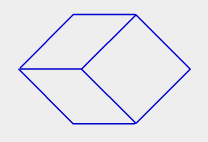
\includegraphics[scale=1]{QuickPic1}
\quad

\includegraphics[scale=1]{QuickPic2}



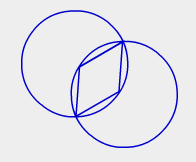
\includegraphics[scale=1]{QuickPic3}
\quad

\includegraphics[scale=1]{QuickPic4}



\includegraphics[scale=1]{QuickPic5}


Here is another optional in-class activity for leading off the geometry chapter (or for use any time during the course of the chapter).  The activity is described below.  

\begin{itemize}
\item
Students should work in partners, and decide who is Partner A and who is B.  

\item
Everyone gets a couple sheets of dot paper (you can get some here: \url{http://www.printablepaper.net/category/dot}).  Put up some kind of divider between the partners so they can't see each others' work.

\item
Give everyone a few minutes to create a simple design on the dot paper.  

\item
Partner B sets aside his drawing for a moment and gets a blank sheet of dot paper.  Partner A describes her drawing to Partner B using just words (no gestures, no showing the drawing, no correcting what Partner B draws).

\item
Partner B tries to re-create the drawing as accurately as possible from the description.  He can ask yes / no questions, but no other clarifying questions, and he cannot show his work until he thinks it is complete.

\item
The two partners compare the original and the copied drawing to see how they did.

\item
Switch roles: Partner B describes his drawing while Partner A re-creates it.
\end{itemize}

End the activity with a whole-class discussion: What was easy / hard about the activity?  What words did they use to communicate clearly?  What kids of drawings were easier to describe or harder to describe?  The idea is to see that mathematically precise language (``draw a square two units on each side with sides parallel to the sides of the paper\dots at the midpoint of the top side of the square is the vertex of a right triangle, and the other two vertices are ...'' versus ``it looks kind of like a flower but the petals are more pointed and not round'') helps you to create the drawing accurately and convey locations and relationships precisely.


After either (or both) of these warm-up activities, move on to the Think / Pair / Share on page 1 and  a general discussion of what it means to study geometry.  Focus on the idea that geometry is more than just naming and classifying shapes, but it means understanding and reasoning just like other areas of math.  

In the discussion about the objects (point, line, plane, etc.), ask follow-up questions: how is a point different from a dot on the page or on the blackboard?  (A point is an \emph{abstraction}, just a location.  We could never actually see a point because it doesn't have any length or width.)  Same for a line: how is the mathematical idea different from what we draw on the page?  Is a piece of paper really a \emph{plane}?  How come you can never draw a true circle?  The idea is to emphasize that the drawings we make in geometry are just aides to our reasoning, but they should not be taken as truth.  








\subsection{Tangrams}
\subsubsection*{Materials:}  You can get plastic tangram sets for use in class, or simply ask students to make a copy of the tangrams (careful tracing is OK, but a photocopy is better) and cut out the pieces before the in-class activity.

\subsubsection*{Activity:}
This activity gives you a chance to review a lot of geometric vocabulary in the context of solving problems.  It is probably best to allow the vocabulary to come up naturally in context, perhaps keeping a running list on a side board.  Encourage students to copy  down the list before the end of class so they have a record of the terms that were used, but do not over-emphasize naming as the fundamental idea in geometry.

Ask students to work individually on Problem 1.  When a few students have finished,  one of them can demonstrate a solution to the class, and  everyone who did not yet solve it can   create the square with their own tangram set.  Encourage students to trace around the individual shapes to record their solution.  Ask the class how they know the final object is a square: How do they know the angles are right angles (this depends on what we assume about the original tangram pieces)?  How do they know the sides are all equal (again, this depends on some properties of the tangram set)?

Tell students that for the purpose of working with the tangram set, sides that appear to be equal will be considered equal, and angles that appear to be right angles will be considered to be so.  

The students can then work on Problems 2 and 3, and follow the same strategy of presenting, recording, and justifying solutions.  You may wish to demonstrate how you can take the solution for a square and turn it into one for the non-square rectangle by just moving two pieces.  

\begin{center}
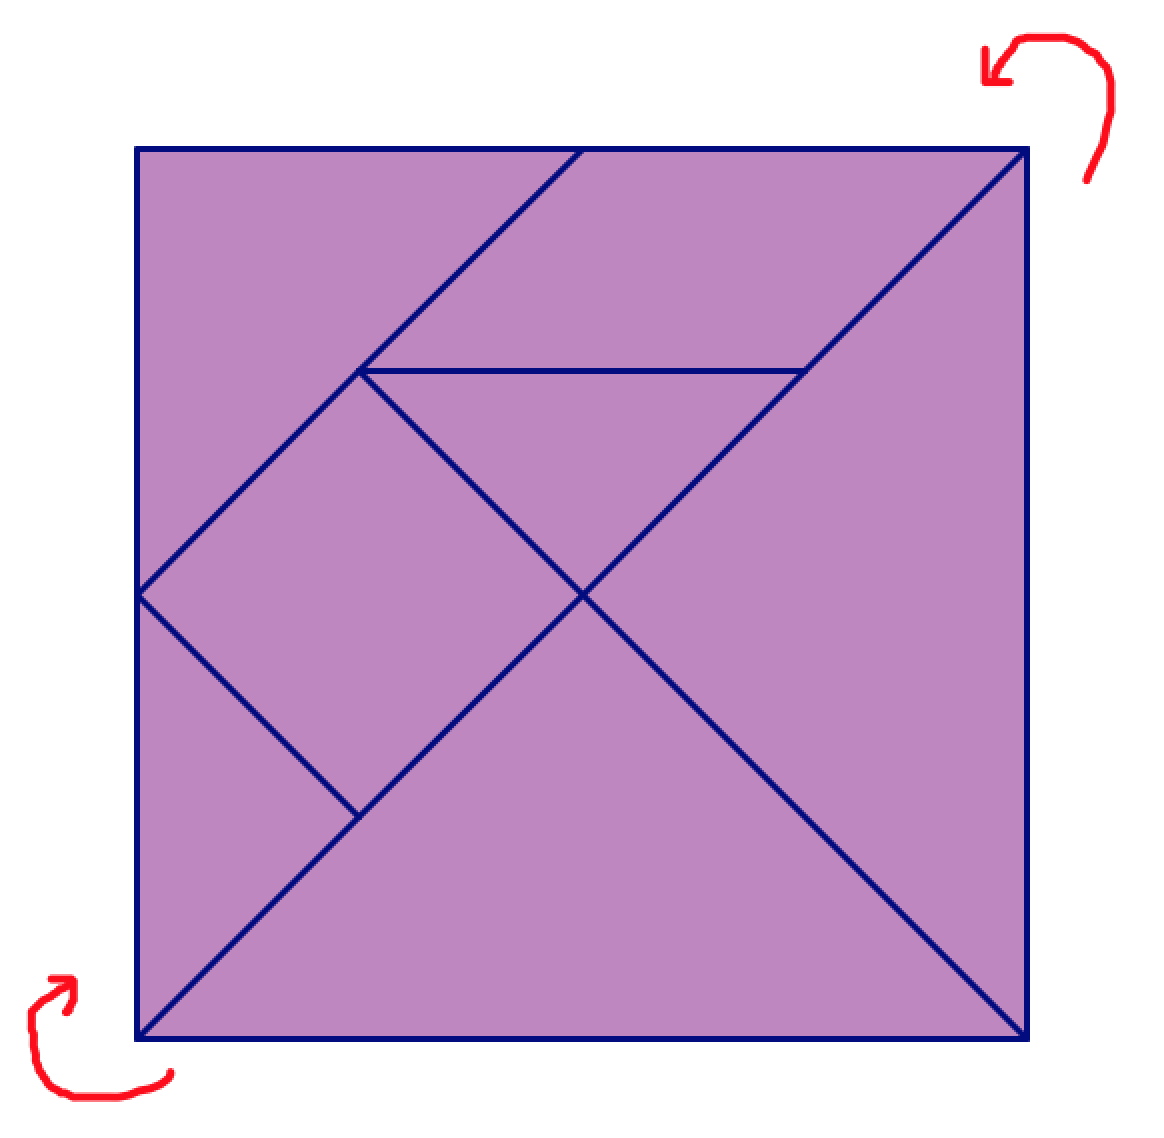
\includegraphics[scale=0.25]{squaretorect1}
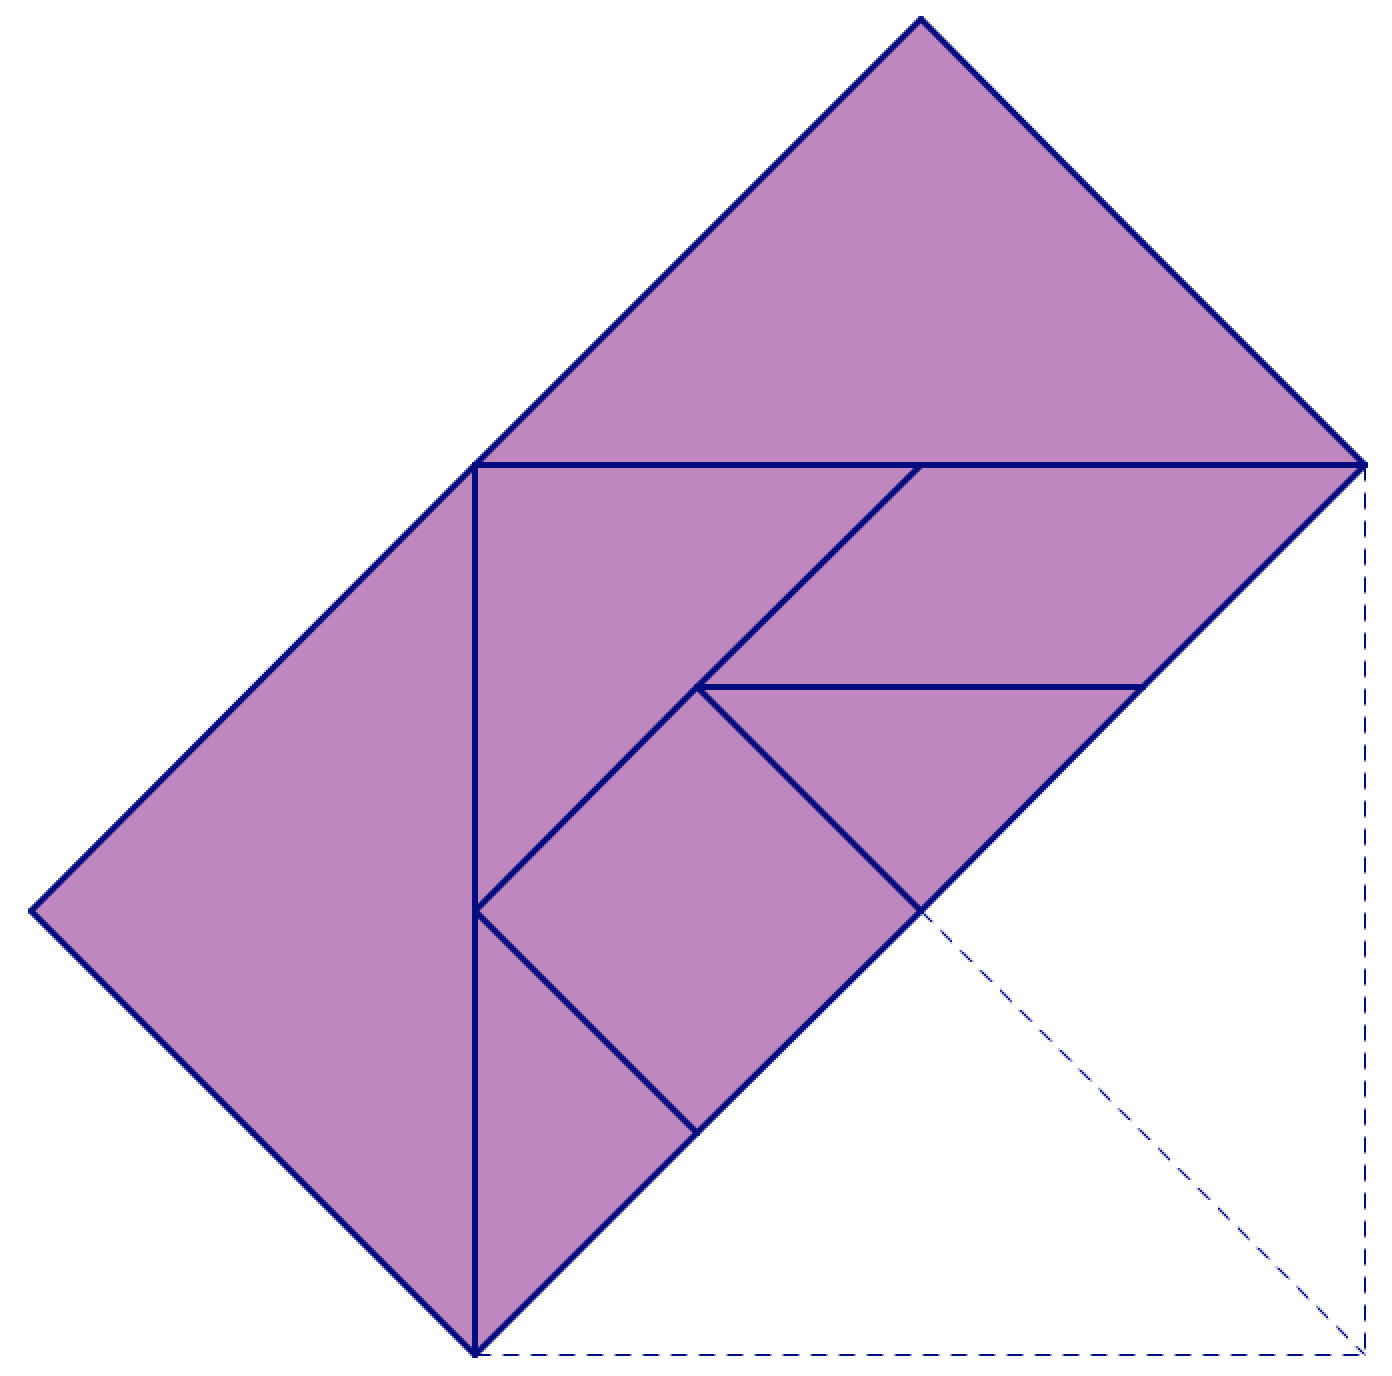
\includegraphics[scale=0.25]{squaretorect2}

\end{center}

A similar trick turns the square into a right triangle.

\begin{center}
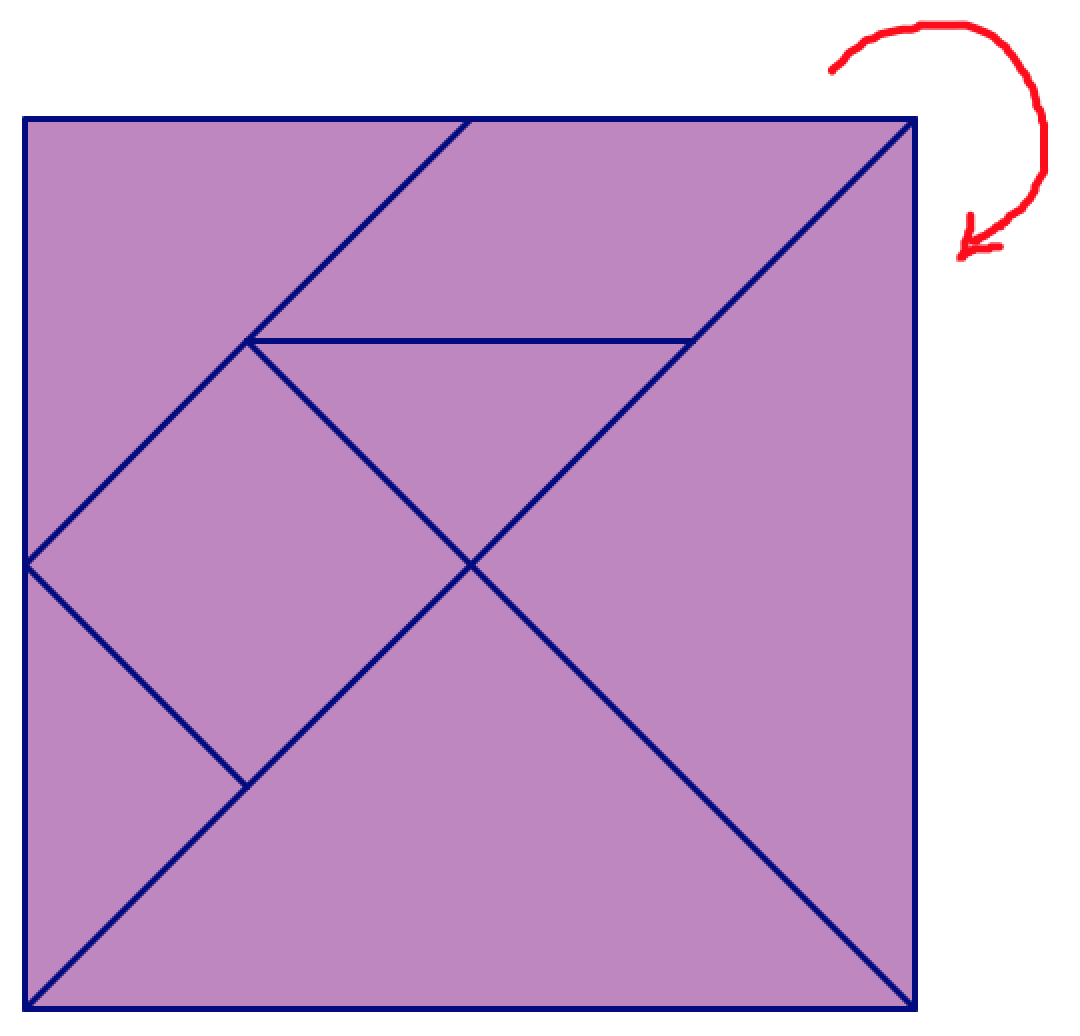
\includegraphics[scale=0.2]{squaretotri1}
\quad
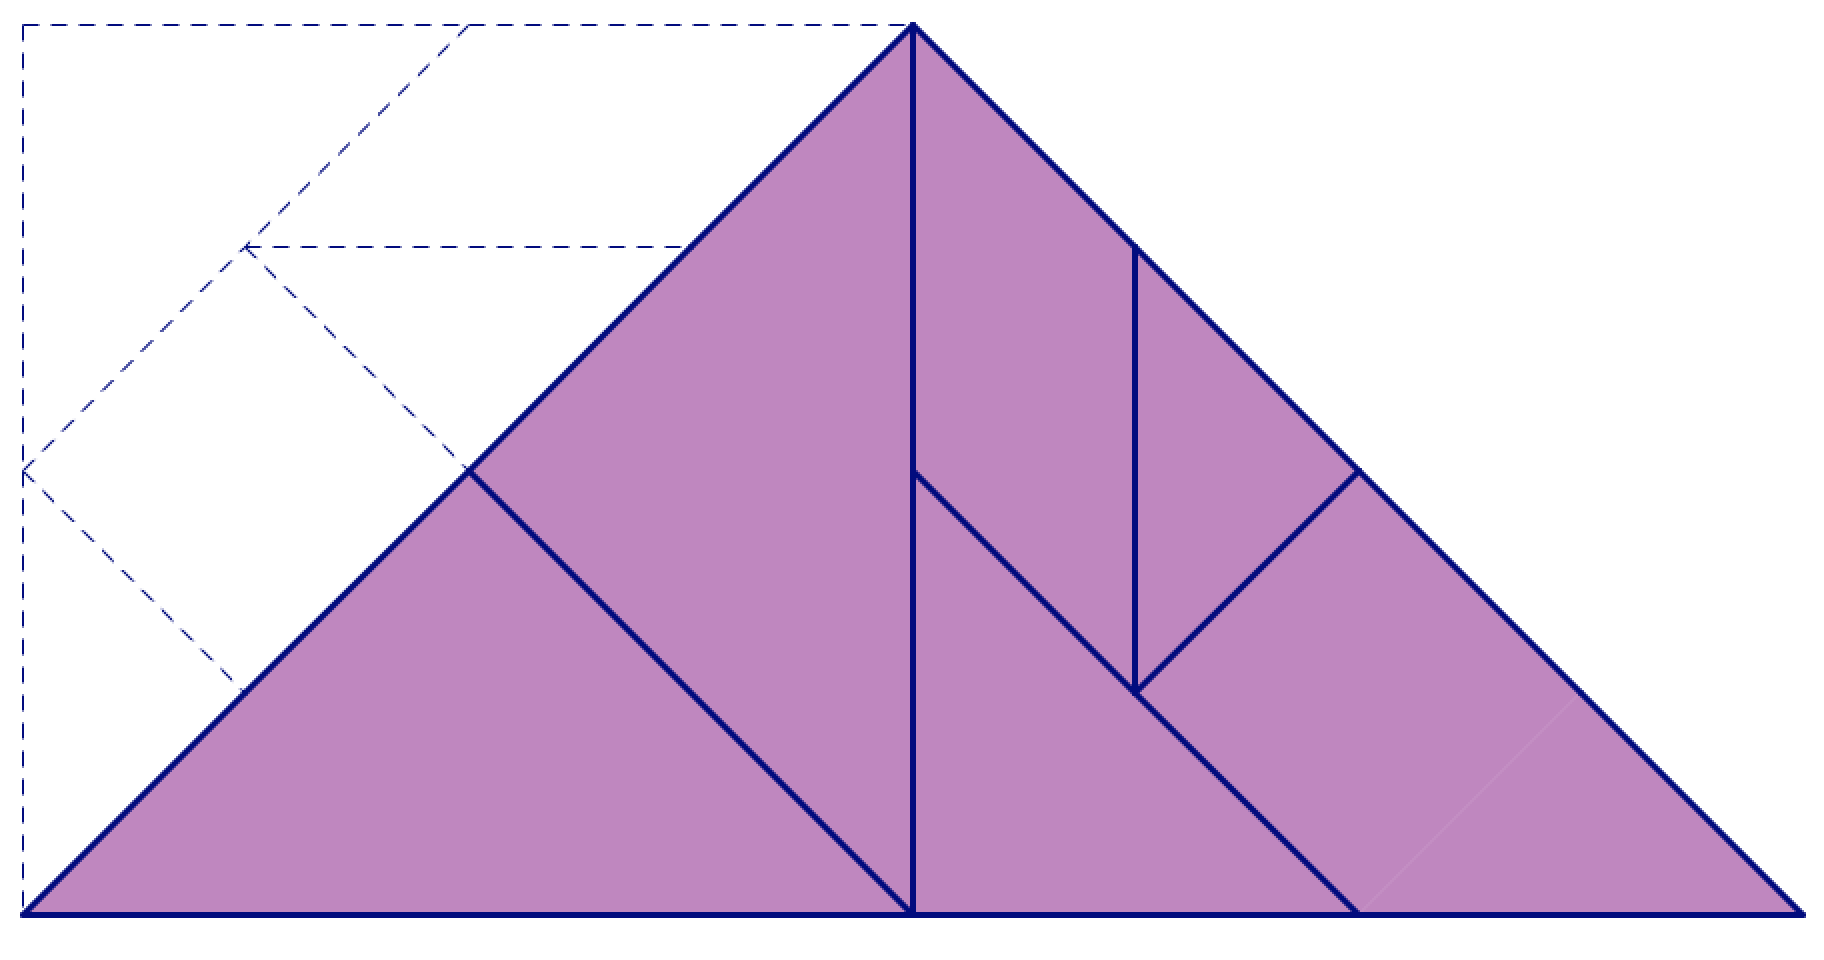
\includegraphics[scale=0.2]{squaretotri2}

\end{center}


You can point out that visualizing these kinds of decompositions can be very useful in reasoning about shapes in the early grades, leading to area formulas and more in later grades.

Allow students to work at their own pace on Problem 4.  If you wish to have extra puzzles for students who finish more quickly, you can find lots of additional puzzles online, including some with solutions shown.  

Finish the activity with the Think / Pair / Share on p.4.  Students usually find making the human and cat figures easier than making the more abstract figures because  the locations of one or more of the tangram pieces is usually obvious, and the rest can be built from this first clues.

Problem 20  in the Problem Bank would make appropriate homework  at this point or any time after.  You can also ask students to create tangram puzzles by making a design with their seven pieces and tracing just around the outside of the design.  You can then use these puzzles in class or for additional homework later in the chapter, where students solve the problem and then around the individual tangram pieces to show the solution.



\subsection{Triangles and Quadrilaterals}
\subsubsection*{Materials:} Before the triangle inequality activity (section 2.2), you will want students to copy and cut out the strips of paper on page 12.  As an alternative, you can use linkage strips if you have them available (\url{http://www.diytrade.com/china/pd/9525966/Math_Linkage_Strips_Toy.html}).  There are online versions of this activity available as well, so an alternative would be to assign that as homework or do the online version in class if the students have technology available.  An interesting conversation for future teachers would be whether they find the online  activity as convincing as working with physical materials.  Do they trust the computer as much as their own hands and eyes, or do they wonder if the outcome of the activity is just an artifact of how it was programmed?  See \url{http://www.learner.org/courses/learningmath/geometry/session2/part_b/index.html} and \url{http://www.learner.org/courses/learningmath/geometry/session2/part_b/constructing.html}.


\subsubsection*{Activity}
The Think / Pair / Share on page 5 can be done as an instructor-led activity, with students comparing their work with a partner after having drawn all five triangles.  They should articulate to their partner what makes each of their triangles different from each other.  Then discuss as a whole class what makes triangles ``different.''

If if doesn't come up in the discussion, you may want to propose your own solution: Draw five equilateral triangles of varying sizes and ask if the class thinks you have followed the directions given.  There will likely be some disagreement on the matter.  Use this opportunity to point out that ``different'' is not a precise mathematical term.  You can introduce the terms ``congruent'' and ``similar,'' and have the class come to agreement on whether similar (but not congruent) figures are different or not.  You may want to point out that throughout the text, ``identical'' means ``congruent.''  

The classification of triangles can be drawn out of the group discussion, where you point out that you can change size (similarity), angles, or sides of a triangle to cause differences.  Ask students what types of triangles they know, and point out when a name refers to classification by sides versus by angles.
As in the previous activity, the vocabulary can be put up on a side board and copied by students before the end of class.


Return to the Poincar\`e quote that geometry is the art of good reasoning from bad drawings.  Note that when working in geometry, we often make \emph{sketches} to aid our thinking and not \emph{careful drawings}.  So we can never solve problems by saying one side looks longer in a picture, or it appears that three lines intersect in a point.  We use the drawings to get ideas, but always must reason through what is really true.  Introduce the use of tick marks, and emphasize that tick marks and measurements given in the drawing of a problem always overrule what your eyes say is true.  You may want to draw some obviously bad examples to illustrate this point.    Follow this introduction with the On Your Own exercises, either in class or for homework.
 Other homework that can be assigned anytime after this point: Problems 21--24 in the Problem Bank.
 
 

\subsubsection*{Angle sum}
The angle sum activity is a quick follow-up to the ``different triangles'' activity.  The reason for having students tear (rather than cut) the angles off the triangles is so that they can recognize the original vertices of the triangle.  An alternative would be to have students put a dot of ink inside each vertex before tearing or cutting it off, so they are sure to put the correct three vertices together.

This activity serves to both remind students of the fact (which they certainly learned at some point) that the sum of the angles in any triangle is $180^\circ$ and to remind them of our focus on reasoning and explanation.  Of course, since the angle sum in a triangle is equivalent to Euclid's fifth postulate, the ``explanation'' here is perhaps a bit less satisfying.  You can offer the standard proof based on parallel lines and alternate interior angles if students are curious, but in fact it's just a matter of which version of the fifth postulate you choose.

\begin{center}
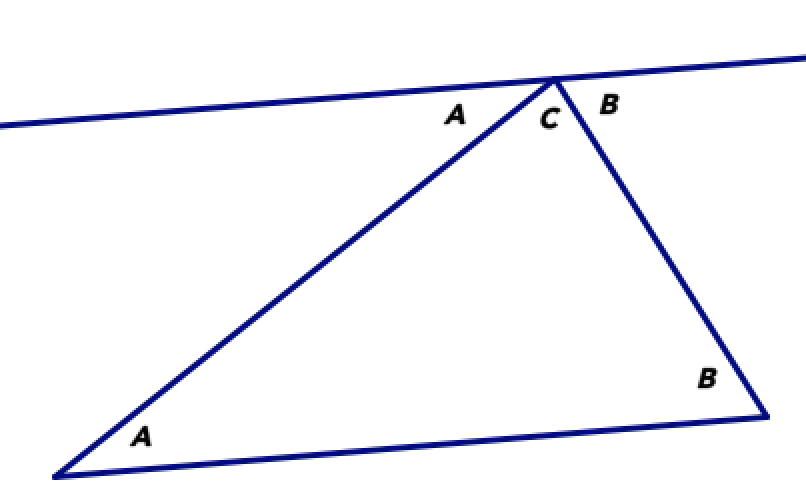
\includegraphics[scale=0.5]{triproof}
\end{center}

If you have a beach ball or globe, you can demonstrate the fact that this statement is false in spherical geometry, emphasizing that it's an artifact of the geometry we usually study in school --- the geometry of a perfectly flat plane.

The final reading covering these ideas could either be done as a brief lecture, as a homework assignment, or as student-led reading with students taking turns reading sections of the text.

Anytime after this point, Problem 25 in the Problem Bank is an appropriate homework assignment.





\subsubsection*{Triangle inequality}
Students should have cut out strips of paper of various unit lengths.  Anyone who doesn't have the strips must partner with someone who does.  
Once they are in  groups: First ask them to pull out their strips and group them: which are one unit long?  two units?  three? four? five? six?  (They should have at least three of each length.)

Explain to the students that they will be building triangles from their unit strips.  You may want to demonstrate how to use the strips to build a triangle with no overlapping or folding allowed.  The strips must just touch at the inside corners, so that the length of the strips accurately reflect the lengths of the triangle's sides. 

 
To launch the activity, ask groups  to take one strip each of lengths 4, 3, and 2 units and try to make a triangle with the strips.  Decide if it's possible.  Walk around the room to be sure students have used the strips correctly.  Repeat with lengths of 4, 2, and 1 units.  Make sure everyone sees it's not possible.   Students can then work for several minutes to try lots of possibilities and keep track of their data in a table.  Emphasize that the goal is to be able to form a general rule.  Given three lengths, you want to know if it's possible to build a triangle or not, without having to cut out the strips and try it by hand.

Bring the class back together and ask them to generalize their findings by answering the two Think / Pair / Share questions on page 13.  Then ask for their general statement and an explanation.  They may have visual / kinesthetic ideas like two arms of the triangle reaching out for each other and trying to touch, but not being able to do so if they are too short.  

A more geometric explanation would be to draw one side of the triangle and then circles of the appropriate radii at the endpoints (representing swinging the other two sides around to every possible position).  If the circles don't intersect, no triangle is formed.  If you have access to dynamic geometry software like Sketchpad \url{http://www.keycurriculum.com/}, the demonstration is even more convincing than a static picture.

\begin{center}
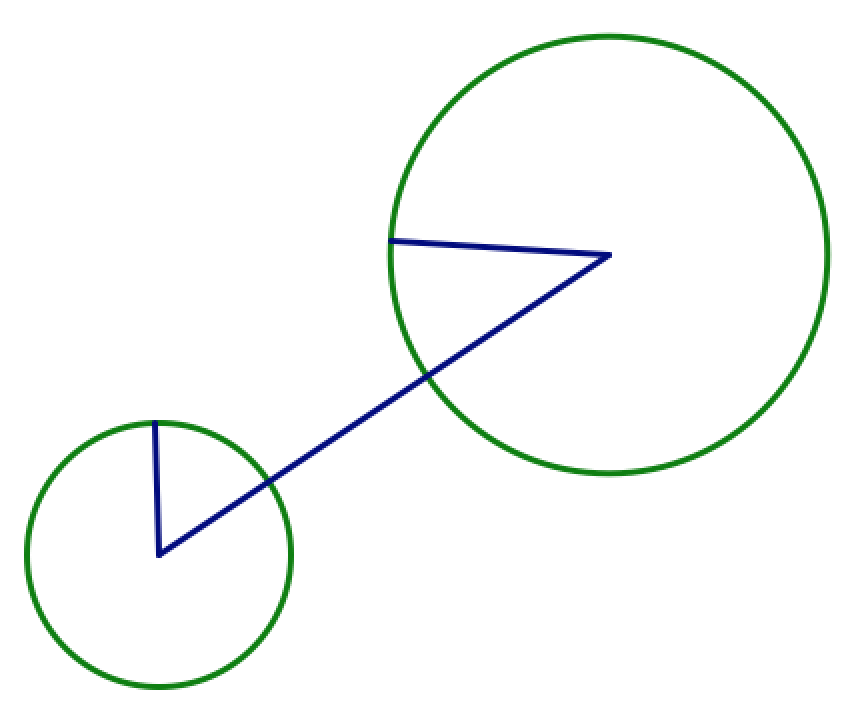
\includegraphics[scale=0.5]{trienqcirc}
\end{center}

Make sure the discussion leads to a careful statement of the triangle inequality and a reasonable explanation.


After the conversation about the Triangle Inequality, ask students to work on Problems 6 and 7 with their partners.  It should not take long for them to realize that if three lengths form a triangle, they form a unique one (SSS congruence), but if four lengths form a quadrilateral, they can form many different ones.  The explanations on pages 16--18 can be drawn out of the class discussion, covered as a lecture, or assigned for reading.

As an alternative, you can ask students to do this activity online for homework (see the \emph{Materials} section above) and then have the class discussions (about both the Triangle Inequality and SSS congruence) at the start of the following class.  

After you've covered the triangle inequality, Problems 26 and 27 are appropriate for homework.  Any time after the end of this whole section, Problem 28 is a good homework problem.  With each of these (especially Problem 28), you probably want to devote some time in class to discuss students' work either before or after grading it.  On Problem 28, students may indicate mistakes based on how things look in the picture (for example, ``$DC$ is shorter than $BC$, but the drawing says that $DC$ is 8 units and $BC$ is 5 units...'').  Emphasize that they need to reason through what they know (angle sum, triangle inequality, SSS congruence) and use those facts, not use how things ``look'' in the drawing, to find the errors.

Problem 29 could also be assigned at this point, but is probably more appropriate after students do the in-class activity on constructing towers (Section 7.1).






\subsection{Polygons}
As an alternative to having students read the definition in class and create examples and non-examples, you may wish to work the other way: ask students what they know about polygons and have them create a working definition.  Provide non-examples that still fit their definition, and have them revise and refine the definition until it works.  This activity --- creating a precise mathematical definition --- is an important part of doing mathematics, and not something we let our students experience often enough.  It is a worthwhile activity.

Emphasize to students that when they think about polygons for the rest of the chapter, their mental images should include not just regular polygons, and not just polygons oriented in a particular way.  They should be sure to think about all kinds of polygons unless the problem says otherwise.

Students can work individually or with a partner on Problem 8.  You may want to  demonstrate with one of the designs (Design 2 is a good choice) that there are some non-obvious ``hidden'' polygons.  Tell students their job is to find all of the polygons in each design.  They will have to come up with some way to keep track of what they have and haven't counted.

Conclude the activity by asking students to share their answers and compare their work when there is any discrepancy.  Ask students how they kept track of their work and avoided double-counting.  Some of them may have made multiple copies of the designs with the different polygons shaded.  Others may have used something like the standard scheme of assigning letters to vertices and writing down the names of polygons as they were found.  In either case, they have to worry about noticing a double-counted polygon and a systematic way to find them all.  Some might look for all triangles, then all quadrilaterals, etc.  Others might use a ``negative space'' approach: finding a triangle, and then whatever polygon is the complement of that triangle in the design, and so on.  

The activity on angle sum in a polygon and the measure of each angle in a regular polygon are short in-class activities (or a combination of in-class for the angle sum and homework for the regular polygons).  The main purpose is twofold: First, those facts will be useful to students in the upcoming activities on Platonic solids and on tessellations.  Second, it again allows us to focus on how we can use reasoning to explain and justify our work in geometry.  We could, of course, measure angles in various polygons and guess at an angle sum based on experiment.  But the simple act of cutting polygons up into triangles allows us to create a convincing explanation of the angle sum formulae that avoids issues of not being able to test every case and of the precision of our measurement tools. 

The text does not focus on the proof that any $n$-gon may be cut into exactly $n-2$ triangles.  You may decide that you want to help students create a justification of this statement as well.  It is essentially an inductive proof.  Find three adjacent vertices where the diagonal between the two outer vertices is inside the polygon (this is always possible if $n>3$ because we don't allow self-intersection).  Draw this diagonal to form a triangle and an $(n-1)$-gon.  Now repeat.  





\subsection{Platonic Solids}
\subsubsection*{Materials:} You can find snap-together polygons like Polydrons \url{http://www.polydron.co.uk/} or ones that connect with magnets like these \url{http://www.magformers.com/}.  If you don't have access to these materials, simply ask students to copy and cut out the regular polygons as directed on page 25 before the in-class activity and provide them with tape.

\subsubsection*{Activity}
The in-class activity is outlined in the student notes.  Because the materials can be tricky for a single person to work with, the activity is most easily done with groups of two or three students working together.  You may want to check in periodically with what students have found.  In particular, many students incorrectly complete the icosahedron.  Starting with five triangles around a vertex taped together, students may create two copies of that ``cap'' and tape them together.  Point out to students that all of the other vertices have only four triangles meeting, so it is not a regular polyhedron.  Ask if they can fix the construction so that five triangles meet at \emph{every} vertex.

The theorem statement and the proof (Problem 11) can be drawn out of a whole-class discussion after the activity.  Remind students what they know about angles in regular polygons to create their justifications.



\subsection{Painted Cubes}
This is best done as an in-class activity in small groups.  If you have snap-cubes or other materials to bring to class, you may want to encourage groups to actually build the  $2\times 2\times 2$, $3\times 3 \times 3$ and $4 \times 4 \times 4$ cubes as a warmup, and then use those cubes to help with their investigation of the painted cube problem. 

If students work in groups, you may want to give each group poster paper or a place on the board to display their findings, and then allow groups to either present their work to the class or walk around and look at everyone's work before a whole-class discussion and wrap-up.

This activity connects back to the first chapter on algebraic thinking.  As in that chapter, students should focus not just finding a pattern in the painted cubes (there are actually several patterns to find), but also in describing the patterns using correct mathematical symbols, and most importantly explaining why the patterns are correct based on the problem situation.


\subsection{Symmetry}
\subsubsection*{Materials:} The activities in this section can be with just blank paper (tracing paper is useful but not necessary) and the text.  If you have access to Miras (\url{http://www.enasco.com/product/TB14953T}), you may want to bring them and incorporate them into the ``Line Symmetry'' activity (Section 6.1).   Alternatively, you may wish to bring a variety of materials (rulers, protractors, compasses, string, measuring tape,  tracing paper, colored pens, etc.) and simply tell students: ``I have a bunch of tools that might be useful for you.  If there's something you want to use, ask me.  If I have it, I'll give it to you.''  This encourages students to think for themselves what tools are appropriate and useful, rather than following your lead for what to use.  (Note: CCSS Math Practice 5 is ``Use appropriate tools strategically.''  The idea is for students themselves to decide which tools --- both physical and mathematical tools --- are appropriate to a given task and to use them well.)


\subsubsection*{Activity:} 
After launching the activity with the Think / Pair / Share on pages 32 and 33, students can work individually or in groups on Problems 14 and 15.  One way for students to complete Problem 15 would be with tracing paper: Trace the design including the line of symmetry, then flip over the paper and match up the lines.  They could also use folding along the line and tracing.  Students may come up with other ideas.  You can ask them to share their methods and discuss whether they think their method produced a fairly accurate design (like the methods above) or whether it was inaccurate (just ``eyeballing it,'' for example).


The activity on rotational symmetry (Section 6.2) follows a similar structure.  In the Think / Pair / Share, focus on the question of how the angle of rotation corresponds to the number of turns you can do before coming all the way back around.  Again, tracing paper may be useful.  Students may want protractors or another method of measuring the angle of rotation.  You can also  have them think about how they could use folding to create an accurate $90^\circ$ or $60^\circ$ angle if protractors are unavailable.


The final activity on translational symmetry could be done as a short in-class wrap-up or as a homework assignment.   Problem 30 is also an appropriate homework assignment at this point.



Other in-class activities and homework: You may want to bring in objects with symmetry with some cultural significance (for example, traditional printed fabrics from various cultures, if you have access to them).  Students could explore the question of whether different types of symmetry are more prevalent in the traditional arts and design some cultures rather than others.  Or you may assign a ``symmetry scavenger hunt'' homework problem, in which students must bring in objects or pictures of objects from their home or neighborhoods that show symmetry, as well as objects that do not show symmetry.  They can share these objects in small groups or with the whole class, including describing the symmetries they have found.

Homework problems could also include creating their own designs with line symmetry, rotational symmetry, or translational symmetry.  You can specify the problem more, for example ``Create a design that has exactly three lines of symmetry,'' or ``Create a design with line symmetry but no rotational symmetry.''

As a larger homework assignment, you can ask students to create a geometric ``Matching Game'' like the ones they played in Chapters 1 and 2.  They will have to decide on what goes on the cards (shapes, names, descriptions, symmetries, etc.) and create the cards to turn in.  You could then use the cards for a future class activity, or just have students swap cards with a partner and try each others' games out.



\subsection{Geometry in Art and Science}
\subsubsection*{Materials:}
The activity on Tessellations (Section 7.1) requires that students copy and cut out the shapes on pages 42--47 before the class activity.  The activity on Escher drawings (Section 7.2) requires large poster paper for each student, crayons or markers (you may ask students to bring their own if you do not have them), and some stiff material like cardboard or stiff poster paper (even old file folders will do), and you may want to bring large copies of the square, equilateral triangle, and regular hexagon to trace onto the stiffer material.  You will also need scissors and tape, though these can be shared by the class.
The ``Building Towers'' activity  (Section 7.3)  requires a large amount of toothpicks and mini marshmallows.  (These are really the best materials to use.  Alternatives like gummy candies are more sturdy, and students may not see the utility of triangular supports in their constructions.)  You will also need rulers (preferably yardsticks) or measuring tape.   

\subsubsection*{Activity:}
Geometry certainly began as a very applied field of mathematics, and it's still a helpful way to think about the world around us, including its use in both art and engineering.  This is also an opportunity to bring up some ethnomathematics, especially in regards to how different cultures use geometry in their buildings and communities.  (For just one example, see the TED talk by Ron Eglash here: \url{http://www.ted.com/talks/ron_eglash_on_african_fractals}.)

The section consists of three in-class activities, each of which is described fairly carefully in the student chapter.  The ``Building Towers'' activity should not take a full class period.  Focus the debriefing conversation on what students learned and what they would do differently.  It is very likely that many groups try to build a tall rectangular building like a skyscraper, but with these flimsy materials, those will collapse quickly under their own weight.  The groups who use wide bases and triangular supports throughout tend to have more successful designs.  You may wish to demonstrate this idea specifically by having each group build a tetrahedron and a cube out of the toothpicks and marshmallows, and see how easy it is to squish the cube flat, compared with how strong the tetrahedron is.  

If there is extra time, you may want to give students the chance to re-do the activity (maybe with a shorter time frame) and see if, based on what they learned in the discussion and from experience, they can do a better job the second time.  Instead, you may want to combine this activity with wrapping up some earlier work.

The tessellations and Escher drawing activities can be combined into a single 75-minute class session (students may need to complete the Escher drawings at home).  A shorter class session may require splitting the two activities over two days.

Note that the directions in the student materials just have students cut out a design from one side of their base shape and move it to another side via a translation or rotation.  Of course, you can do this multiple times (say on opposite sides of a square), or even cut a design from half of a side and move it to the other half of that same side.  A longer tutorial is here: \url{https://www.youtube.com/watch?v=212XC1zfxXY}.  You may want to share this video with students, or use it for inspiration in taking the in-class work farther.
 

After the ``Building Towers'' activity, you may want to assign Problem 29 from the Problem Bank, and spend some time in class with students sharing their pictures with the whole class.


\subsection{Problem Bank}
This section contains problems to be used for homework and quizzes, or for additional in-class activities.  Specific suggestions for which Problems to use with which Sections can be found above in the notes for each Section.










\newpage

\section{Chapter 4:  Voyaging on \Hokulea}

Our students are future elementary school teachers, so they will most likely teach all subjects to their students.  We'd like to help them think about seeing mathematics --- and asking mathematical questions --- in contexts that don't come straight from the math book.

Many schools in \Hawaii\ encourage teachers to include learning experiences that deal with the history and culture of the people who originally settled these islands, including their descendants and how they lived.  There is actually a tremendous amount of mathematics that could be brought out for elementary students in these lessons, so in this chapter we give our students one glimpse of how this can be done.

The whole chapter will take approximately two weeks of class time, but you can pick and choose from the activities to make the chapter longer or shorter.  

You can find a lot of information about voyaging on \Hokulea\ at the Polynesian Voyaging Society website \url{http://hokulea.org/} and \url{http://pvs.kcc.hawaii.edu/}.   Particularly useful is the FAQ and ``ask the crew'' site: \url{http://www.hokulea.com/education-at-sea/ask-crew-question/}. What follows is a suggested outline for working through this unit with your class, along with some relevant details that may help you in your teaching.  (Note: There is a ton of information online about \Hokulea.  If students ask you something that you can't answer, ask them to research it and find out!  Remind them that you are not a voyaging expert but a mathematics expert, so your job is to provide just a bit of context and then help them with the mathematical part of the lesson.)


\subsection*{Flow of the unit}
This section presents one suggestion for how to manage about two week's of class time  (based on a MWF schedule).  Note that each day you will check in on their progress on the project.  This is really to keep their focus on the project (Problem 3 in the chapter) and encourage them do a bit each day.  It should not take a large amount of class time, unless there are significant stumbling blocks you feel you need to address.  The goal is to just make sure they are making progress and on the right track, and to loin them to any resources or ideas they will need.

\subsubsection*{Day 1}
Ask students to read the first page and talk with a partner about the Think / Pair / Share questions.  Generate a long list of mathematical problems and  questions they have about voyaging.  Keep encouraging them to ask more questions.   You may need to throw in some of your own questions to get them going.  (How big is the canoe?  How many people are on it?  How long are the voyages?  Where does the crew sleep?  How is it powered? \dots They probably know almost nothing at this point.  Of course, you may find that one or more of your students knows a lot about \Hokulea, so let them become the class expert, answering questions whenever they can.)  You probably want to keep a record of these questions somewhere and come back to them on Day 3.

Some history that you may want to share with your students after the conversation:  The ``accidental drift'' theory was shot down by computer simulations of wind patterns and ocean currents which concluded that a drifting canoe had no chance of reaching \Hawaii, Easter Island, and New Zealand from other parts of Polynesia or Micronesia.  





The route between Tahiti and Hawaii passes through three ocean currents and requires sailing slightly against the wind both ways. Could the ancient voyaging canoes perform well enough to windward to make round trips? \Hokulea's 1976 round trip voyage proved that they could. And the navigation experiments conducted in 1976 and in subsequent voyages have proved the adequacy of Polynesian navigation.

Also: Wilford, John Noble (18 January 2008). ``Pacific Islanders' Ancestry Emerges in Genetic Study''. Asia Pacific (The New York Times Company):  DNA analysis confirms Polynesians' relationship to Taiwanese Aborigines and East Asians.


After the discussion, students can work on making the scale drawings and the computation of how much space everyone gets.    They should finish this for homework if they do not finish in class.  You may want to bring tools for them to use (calculators, rulers, protractors, etc.)  

For additional homework, ask students to read all of Section 2, including reading the linked web page and watching the video (or you may choose to show the video in class instead, at the start of Day 2).  Emphasize that they don't need to work on the problems, just read everything over before class so they have seen it.




\subsubsection*{Day 2}
 At the start of class, explain that Problem 3 (the report for the quartermaster) is a project to cover the whole rest of the unit.  They should work on it a bit each day.  You will check in with them at the start of each class, and they should have something to share with you (and the class) about what they've done, or they should have clarifying questions to ask of you.  
 
 As the instructor, you should decide on the format of the report (must it be typed? any other specifics you want to give them?) and let them know that up front.  Encourage students to work out everything in a notebook, keeping track of their ideas, and then write the formal report at the end, once they have worked everything out.  Before the next class, they should choose their leg of the voyage and at least make an attempt to compute how long the trip would be. 

 The details of the provisions given in the unit are drawn from  \url{http://pvs.kcc.hawaii.edu/ike/canoe_living/modern_provisions.html}.  You can find more details there as well, and you can decide how much of the additional details you wish to share with your students.  We intentionally left out details that we felt were either too confusing to include or that did some of the calculations we wanted students to do.  You may, of course, make different instructional choices.  

For the in-class activity: Have students compare their scale drawings of \Hokulea\ with each other.  Note that the directions did not say what scale to use, so students likely made very different choices.  There was also a lot they didn't know gut could estimate, for example exactly where the deck is placed relative to the front and back of the canoe and how the curvature of the two hulls looks.  You may want to ask several students to share their scale drawings with the class and point out what is good and what could be improved.  An optional homework assignment would be for students to make a better version that takes up most of  whole page, which they will use later in the chapter.

 
 Here is one version of a scale model, for your reference.  The back of the canoe is to the left and the front is to the right in this drawing.
 \begin{center}
 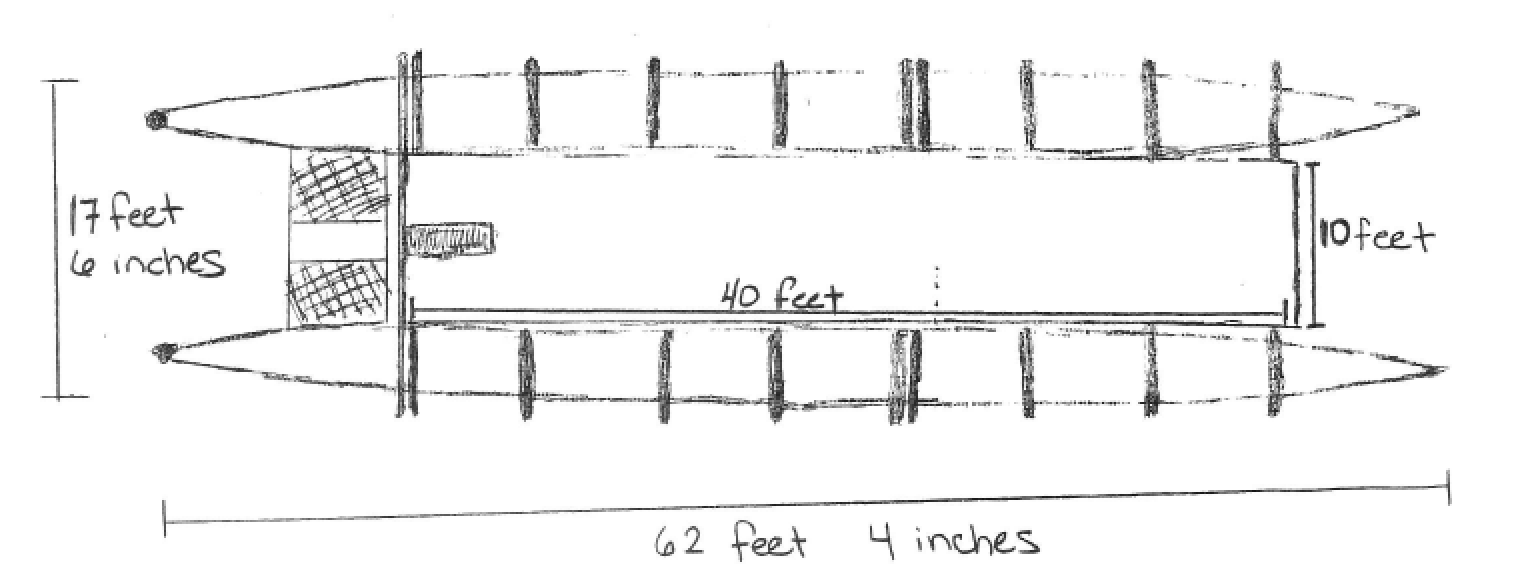
\includegraphics[scale=0.5]{ScaleHokulea}
 \end{center}


Following up on the scale drawings, you may want to take students outside to draw a full-scale model of the \Hokulea. (Bring sidewalk chalk or masking tape to mark off the outline of the canoe,  and bring whatever tools you want students to use: measuring tape, rulers, string, etc.)  When the deck is drawn, ask 12--16 students to all stand on it at the same time.  Ask them to imagine living in this amount of space for the time of a  voyage, say a month or more.  Ask them to just walk around the space and think about how that would feel.  If your class is large, you may want to do this twice with two different groups.  (This may require a second day of class, depending on how long the earlier activities took.)

For homework, in addition to beginning the project, students should read pp. 7--8 and be ready to talk about time-lapse picture of the stars.



\subsubsection*{Day 3}
Check in on students' work on the project.  Everyone should have chosen a leg of the voyage and tried to calculate the time it would take.  Note that the dots on the map provided are possibly not clear enough for students to calculate distances.  They'll need to use a tool like google earth (or an old-fashioned atlas) to figure out where the dot is likely to be and then use that information to calculate distances.

You may want them to just check in with a partner or small group on how they did this and if their methods and their conclusions seem reasonable.  Again, you may ask one or two students to share what they did with the whole class and provide some feedback that could be helpful to everyone.   Take any whole-group questions, and provide assistance or ideas for students who had difficulty.  

Note: You can find a list of \Hokulea's planned ports of call along with longitude and latitude here: \url{http://www.hawaiilink.net/~mms/pvs_wwv/index.php}.  (Scroll below the map on the page for the full list.)  However, providing this list is not as engaging as having students look at the map and figure out where the stops are likely to be.  We provide this information for your reference, but suggest not sharing it with students.  (Of course, some of them may find it in their own research, which is fantastic!)

Similarly, one of our students found a speed-time-distance calculator here: \url{http://www.uspowerboating.com/Home/Education/Navigation/Speed-Time-Distance/Speed-Time-Distance_Calculator.htm}.  Again, we provide these links for your information, but encourage you to let students do some research and find their own way.  Several students opted to use that calculator as part of their final write-up, giving credit to the student who had shared it with the class for the idea.  It is much more meaningful for students to find their own way to this information than to be handed one way to do it. 


For homework, students should revise their route calculations as necessary based on what they learned in class, and they should start the next part of the project:  figuring out how much food and water (in pounds) they and bring.  Students will need to use the information given in the section, along with some estimation.   They should be ready to share their ideas during the next class.


Now that students have drawn a scale model of \Hokulea\ and also (perhaps) had the experience of standing on a full-scale version along with a ``crew,'' they may have additional questions (mathematical and otherwise) that hadn't come up before.  This is a good time to revisit the list of questions they initially generated, cross off any that they know the answer to, and add any new questions.  

The rest of class can be focused on navigation and the initial star compass activity.  Start with a discussion of what they see in the picture of the stars, and why the stars trace out circles through the night.  You might want to point out that stars rise in the east and set in the west, just like the sun.  What maybe is surprising to students is that these circles are all concentric.  They will soon see how this plays in to how navigators figure out where they are in the world while out on the open ocean.


Ask if anyone knows what the bright spot is at the center of the concentric circles (Hokupa\kern.05em`\kern.05em\relax a, the North Star) and its significance for navigation (unlike the other stars, it doesn't move, so you can always find ``north'' by looking for that star).
Note that some of the stars don't really ``rise'' and ``set;'' they just circle Hokupa\kern.05em`\kern.05em\relax a.  All of the stars are tracing out circles, but parts of some of the circles are obscured from our vision by the earth and parts are not.  
 The North Star is pretty close to the horizon here in \Hawaii\.  We're about $20^\circ$ north latitude, which means the North Star is almost exactly $20^\circ$ above the horizon.  (At the North Pole, which is $90^\circ$ latitude, the North Star is directly overhead.  That's why it always shows you which way is north.) 
 
 There's lots more information about the celestial sphere and star positions here: \url{http://pvs.kcc.hawaii.edu/ike/hookele/celestial_sphere.html}.  This is not a major theme of the chapter, but if students are interested and there is time, you might encourage them to dig into more of the details.  Of course, if someone in the class knows a lot about the subject, this is a good chance to let them share their expertise with the class.
 
 Finally, have students begin Problem 4 (rough sketch of the star compass from the written directions).  They should complete it for homework if there is not time in class.  For your reference, you can find several versions of the star compass drawings here: \url{http://pvs.kcc.hawaii.edu/ike/hookele/star_compasses.html}.
 


\subsubsection*{Day 4}
Check in on students' work on the project.    Again, you can have them check in with a  partner or small group and then ask you questions, or you can ask for individuals to share what they did with the whole class and the solicit feedback from the other students and from you.  Essentially, they should do something like the following:  About how much does the crew weigh?  What about their personal gear?  You might remind students about the webpage they read, and that ``\dots crew member allowed one 48 quart cooler'' for their personal belongings, so estimate the weight of the cooler plus belongings.  Then multiply all of that by the number of crew.  They know how much water is allowed for each crew member per day.  How much does water weigh?  How many crew on the voyage?  How many days is the voyage?  Should they bring along some extra in case the voyage takes longer than predicted?  How much extra?  (Again, you can find more detailed answers that the crew actually uses at \url{http://pvs.kcc.hawaii.edu/ike/canoe_living/modern_provisions.html}.  For example: for a 30 day voyage, they bring 40 days' worth of water, and then begin rationing if it looks like they will start to run short.)  

For the next class, students should revise their work on the food calculation as necessary, including addressing the question of the weight of the food they would bring.  How much does an average meal weigh?  How many meals will be served on the voyage?  Don't forget the weight of any packaging, and probably extra water for cooking.
You might want to point out that fresh food will not keep long, so they can bring some for the first few days but then should rely on packaged food.  Remind them also that the crew supplements their diet with fresh fish, with one crew member having the job of setting out and watching fishing lines each day.  If time permits, you may want to talk about how the ancient Polynesians chose their provisions, given that ``packaged food'' was not an option then.  You can find some information to share with them here: \url{http://pvs.kcc.hawaii.edu/ike/canoe_living/micronesian_provisions.html}.  There is also a nice video about provisioning the Worldwide Voyage here: \url{http://www.hokulea.com/hoomakaukau/}.  You may want to share that with your students as they work on their projects, or on the day they turn them in.


Students should start preparing the final version of the project that will be turned in.


The class activity will focus on creating a good version of the star compass.  Have students pull out their rough sketches and check that they seem reasonable (they can do this with a partner).  Then explain the motivation for creating a star compass that is as perfect as possible (or just have students read this in the text) and provide them with whatever tools you wan them to use.  One option would be to have a stash of tools (rulers, protractors, string, compasses, etc.) and tell them that they can ask you for whatever they want to use, and if you have it you'll give it to them.

Instead of doing this in class and on paper, you might want to do the activity outside.   You probably want groups of students (maybe 5--10 in each group) to build the compass.  For each group,  you will need a couple of long ropes and something to mark the 32 equally spaced points along the circle (you can use students' shoes if they are willing, rocks, or other similar objects).  You will want at last five ``special'' objects to mark the center of the circle (the canoe) and the four compass points.  

As students work, the important question is how they know they are creating precise circle divisions.  Most groups will try to find the compass points first.  Remind them that they need to be accurate.  North must be \emph{directly across} from south, and  the same for east and west.  Further, the lines connect NS and EW must meet at $90^\circ$ in the center of the circle.  How can they be absolutely certain that this is the case?  As they work, encourage them to think about the geometry they know and what they can use.  For example, students might 3-4-5 right triangles using a marked unit of length to create right angles, or they might use the standard method of construction to find the perpendicular bisector of the segment connecting north and south.  There are many other methods.

If you do the outside activity (or even the one on paper), it is quite likely that you won't finish in one class period.  Leave the last five minutes of class for discussion, even if that means interrupting them in their work when they are on a roll.  Tell them they will have another opportunity the next day to create a really good star compass.  Brainstorm ideas from the groups how they were using the materials and what they found challenging.  Get as many ideas out as possible.  Then assign for homework a paper-and-pencil version using whatever materials they can find (but not a computer), along with ideas to make the second outdoor attempt go more smoothly.







\subsubsection*{Day 5}
One final check-in on students' projects.  Again, have them share with a partner and then ask questions if anything is unclear after that discussion.  Remind them of the due date and of any special requirements you had.

The class activity should start with a discussion of the utility of the star compass.  Talk about the stars staying in their houses as they rise and set.  Refer back to the time-lapse picture of the stars and show how that can be seen in the picture.  Imagine the stars traveling in big circles while staying in their houses, and get explanations for why that would yield the picture you see.


Let the students try the star compass activity again, putting their ideas into practice.

For homework, they should read to the end of the chapter, and think about ideas for how to tackle Problem 6.  They should be ready to dive into that problem during the next class, which means having their scale drawings of \Hokulea\ with them.



\subsubsection*{Day 6}
Collect the final projects, or remind them of the due date if it is still in the future.

Spend the final class on the problem of how to paint a star compass on the rails of \Hokulea.  (Note: the rails run along the deck of \Hokulea.)  You can decide how much direction to give students in this activity.

One idea is to have a star compass drawing that is only slightly larger than the scale drawing of \Hokulea.   Overlay the scale drawing of \Hokulea\ so that the kilo (navigator's chair) is at the center of the star compass.  Use a ruler or other straightedge to connect the kilo to the marked points on the star compass, and draw a mark where these points intersect the rails of the deck.  (Not all of the markings will necessarily fit, but there are enough of them that the navigator can use them.)  Then repeat this process moving the other kilo to the center of the circle.



\subsection*{Other activities}
Depending on the time and resources you have available, you might want to include additional activities in this chapter, either in-class or optional (perhaps extra credit) out-of-class activities:

\begin{itemize}
\item
Visit the Bishop museum and in particular to see the Planetarium show about navigating on \Hokulea\ (currently called ``Wayfinders: Waves, Wind and Stars,'' and showing at 1:30PM daily, but check the Bishop Museum website for any changes).\\

\item
Invite a member of the PVS to visit your class and answer questions from the students.  Or, if that is not possible, have the class select a small number of their questions to send to a crew member of \Hokulea\ by email.\\

\item
Show some of the mathematically themed videos about \Hokulea.  There are many of them available with a Google search.  For example, this video shows how the crew can estimate their speed of travel while they're sailing: \url{http://www.youtube.com/watch?v=3i2xP4N6mbc}.\\

\item
There may be other activities connected with the Worldwide Voyage, such as virtual field trips or connecting electronically with the crew.  Be sure to check the website \url{http://www.hokulea.org} to see what is going on, and have your class follow the progress of the voyage at \url{http://www.hokulea.com/track-the-voyage/}.

\end{itemize}





\end{document}
  
